%---------------------------------------------------------------------------
%          The Hydra Computer Hardware Description Language
%                    User's Manual and Reference
%                         John T. O'Donnell
%                       University of Glasgow
%                     Email: jtod@dcs.gla.ac.uk
%                  Web:   www.dcs.gla.ac.uk/~jtod/
%                Copyright (c) 2003 John T. O'Donnell
%---------------------------------------------------------------------------

\documentclass[a4paper,openany,fleqn]{book}

\usepackage[dvips]{graphics}
\usepackage{verbatim}
\usepackage{subfigure}
\usepackage{amsmath}
\usepackage{hyperref}

\title{The Hydra Computer Hardware Description Language\\
  User's Manual and Reference}

\author{John T. O'Donnell\footnote{%
  Author's address: Computing Science Department, University of
  Glasgow, Glasgow G12~8QQ, United Kingdom.
  Email: \texttt{jtod@dcs.gla.ac.uk}
  Web: \texttt{www.dcs.gla.ac.uk/\char'176 jtod/}}}

\date{Version 0.1.0 (Draft)\\ October 2003}

%---------------------------------------------------------------------------
% Formatting

\setlength{\textwidth}{14cm}
\setlength{\textheight}{23cm}

\def\plusplus{\hbox{$+\hskip-0.5em+$}}

\newcounter{exercisenum}
\newenvironment*{exercise}
  {\addtocounter{exercisenum}{1}
   \vspace{10pt}\noindent\textbf{Exercise \arabic{exercisenum}. }}
  {}

\def\plusplus{\hbox{$+\hskip-0.5em+$}}

%---------------------------------------------------------------------------
\begin{document}

\frontmatter
\maketitle
\tableofcontents
\mainmatter

\chapter{Introduction}
\label{sec:introduction}

Hydra is a \emph{computer hardware description language} (CHDL, or
just HDL) that helps you to design digital circuits.  It provides a
natural and readable notation for specifying circuits, as well as a
variety of software tools for simulation, analysis and netlist
generation.  Hydra also supports the use of formal methods for circuit
design.  It spans a wide range of levels of abstraction, all the way
from CMOS transistors to complete CPU designs.  Hydra focuses on
digital circuits, and it cannot be used for analogue design.

Like all CHDLs, Hydra is a \emph{textual language}: you specify a
circuit by editing a text file that describes its structure and
behaviour.  This differs from schematic capture tools, which offer a
graphical tool allowing you to draw a diagram of the circuit.  In
general, schematic capture tools may appear more intuitive to
beginners, but CHDLs are more flexible and scale up better to large
and complex designs.  Hydra specifications can be compiled and
executed.  Furthermore, the execution can be run in several different
modes; each mode performs a useful action, such as simulating the
circuit or outputting a netlist (which can be used for automatic
fabrication).

Hydra is a \emph{functional} language.  A pure mathematical function
takes an input and produces an output, and circuits do exactly the
same.  This leads to a more natural style of circuit specification
than CHDLs that are based on assignment statements rather than
functions; the reason for this is that a variety of subtle timing
problems are handled more easily and accuratly with pure functions.

Abstraction is one of the central techniques used in software
engineering, and it is equally effective in hardware engineering.
Hydra supports several distinct forms of abstraction, including black
boxes and design patterns.  By using abstraction, we can keep
specifications reasonably small.  A large and complex circuit will be
described by a modest number of separate specifications, each of which
is self-contained and readable.

Once a circuit has been specified, there are several useful tasks that
Hydra can perform automatically.  The most important of these is
simulation: you provide inputs to the circuit, and Hydra will
calculate the outputs.  Simulating a circuit is akin to executing a
program, and circuit design is much more fun when you can watch its
behaviour.

In order to build a physical circuit using a specification, we need a
detailed description of its components and their interconnections.
This is called a netlist, and it can be used directly as input to a
fabrication facility.  Hydra provides tools for generating circuit
netlists, and these can be used to construct real hardware.

Mathematics can be used in many ways to assist in circuit design.
Taken together, these techniques are called \emph{formal methods}.
Hydra provides a rich and powerful approach to formal methods, based
on a simple form of algebra called \emph{equational reasoning}.
Formal methods can be used to transform circuit specifications to make
them more efficient, to derive specific circuits from abstract
specifications, and to prove correctness of designs.

Most languages (including CHDLs as well as programming languages) are
implemented by compilers or interpreters.  Hydra takes a different
approach: it is implemented by \emph{embedding} within Haskell, the
standard nonstrict pure functional programming language.  This means
that a Hydra specification is actually a valid Haskell program, which
can be compiled and executed by an ordinary Haskell compiler.  Many of
the characteristics of Hydra are inherited from the Haskell language.
For example, the key to formal methods in Hydra---equational
reasoning---is one of the central characteristics of Haskell.
Nonetheless, it's better to think of Hydra as a distinct language, not
simply as a special style for programming in Haskell.

This tutorial contains a number of \emph{exercises} and
\emph{projects}.  The exercises are straightforward, and should take
only a few minutes to solve.  Some of them can be done with pencil and
paper, while others require running Hydra.  The exercises are
important because they will help ensure that you have a full
understanding of the fundamentals.  Please do not skip them!  It's
best to read this tutorial near a computer, and to try out the
exercises as you work through the document.  The projects are larger
exercises that give experience with more realistic design problems.
It's valuable to try them, but you don't need to complete the projects
before reading on.

\chapter{Signals and Components}
\label{sec:signals-components}

This section discusses a simple but crucial idea: Hydra treats
circuits as mathematical functions.  It then goes on to introduce the
basic techniques for specifying simple circuits.

In order to try out the examples in this section, you should launch
Hydra.  Go to the workspace directory where you can save files
containing circuit specifications, and launch Hydra, as explained in
Section \ref{sec:check-installation}.

\section{Modelling Circuits as Functions}
\label{sec:circuits-as-functions}

A mathematical function takes an input and produces an output.  This
is exactly what a digital circuit does (with some interesting
exceptions, more on that later).  

A component in Hydra may have a name, which is an ordinary identifier.
For example, \textit{inv} is the name of the inverter, while
\textit{and2} is the two-input logical and-gate.

A wire is a physical connector between components.  A \emph{signal} is
an abstraction of a wire: it connects components, but we are concerned
only with the logical value on a signal, not with the way it is
fabricated physically.  Signals may have names, which are also
identifiers; typical signal names are \textit{x}, \textit{y}, etc.

\section{Logic Gates}
\label{sec:logic-gates}

The most commonly used logic gates are shown in Tables
\ref{tab:1-input-gates} and \ref{tab:n-input-gates}.

\begin{table}[htbp]
  \begin{center}
    \caption{Logic gates with one input}
    \label{tab:1-input-gates}
\begin{tabular}[c]{ll}
\textit{buf}   & buffer: output = input \\
\textit{inv}   & inverter: logical negation \\
\end{tabular}
  \end{center}
\end{table}

\begin{table}[htbp]
\begin{center}
\caption{Families of Logic Gates}
\label{tab:n-input-gates}
\begin{tabular}[c]{llll}
\textit{and2}  & and3  & and4  & logical and \\
or2   & or3   & or4   & inclusive or \\
xor2  & xor3  & xor4  & exclusive or \\
nand2 & nand3 & nand4 & not-and \\
nor2  & nor3  & nor4  & not-or
\end{tabular}
\end{center}
\end{table}

The simplest way to simulate a logic gate is to give it input signals
of type Bool, which has the values True and False.  Try the following
examples by entering each expression after the prompt and pressing
enter:

\begin{verbatim}
  inv True
  inv False
  and2 False True
  and2 True True
\end{verbatim}

A convenient way to run such examples is to select (Copy) the text in
this file, and then paste it into the window where you're executing
Hydra.

\section{Connections}
\label{sec:connections}

\begin{minipage}{2cm}
\begin{verbatim}
inv x
\end{verbatim}
\end{minipage}

A signal is defined by describing a component along with the inputs
connected to the component.  For example, we could define a signal as
the output of an inverter, whose component name is \textit{inv}, with
input $x$, by applying the \textit{inv} function to the argument $x$
(Figure \ref{fig:inv}):
\begin{align*}
& \mathit{inv}\ x
\end{align*}

\begin{figure}[htbp]
  \begin{center}
    \subfigure[Specification]{
      \begin{minipage}{4cm}
        \fbox{inv x}
      \end{minipage}}
    \hspace{1cm}
    \subfigure[Schematic]{
\includegraphics{../figures/xfig/inv.eps}}
    \caption{Inverter.  The output signal is defined as $\mathit{inv}\
      x$.}
    \label{fig:inv}
  \end{center}
\end{figure}

\begin{figure}[htbp]
  \begin{center}
    
\includegraphics{../figures/xfig/inv.eps}
    \caption{Inverter.  The output signal is defined as $\mathit{inv}\
      x$.}
    \label{fig:inv}
  \end{center}
\end{figure}

Punctuation is not required when applying a component to its inputs.
For example, the two-input logical and gate, \textit{and2}, can be
connected to inputs $a$ and $b$ (Figure \ref{fig:and2}):
\begin{align*}
& \mathit{and2}\ a\ b
\end{align*}

\begin{figure}[htbp]
  \begin{center}
    
\includegraphics{../figures/xfig/and2.eps}
    \caption{Logical and.  The output signal has the value
      $\mathit{and2}\ a\ b$.}
    \label{fig:and2}
  \end{center}
\end{figure}

Parentheses are used for grouping, just as in mathematics.  For
example, suppose we want to define the first input to a three-input
and gate as $a$, the second as the output of an inverter with input
$b$, and the third as $c$.  Since the second input is one signal
described by $\mathit{inv}\ b$ (\emph{not} two signals named
\textit{inv} and $b$!), we need to enclose this in parentheses (Figure
\ref{fig:and3-inv}):
\begin{align*}
& \mathit{and3}\ a\ (\mathit{inv}\ b)\ c
\end{align*}

\begin{figure}[htbp]
  \begin{center}
    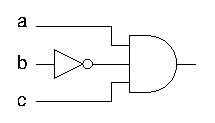
\includegraphics{../figures/xfig/inv-and3.eps}
    \caption{An \textit{and3} gate connected to output of inverter.}
    \label{fig:and3-inv}
  \end{center}
\end{figure}

Figure \ref{fig:andor} shows the output of an $\mathit{and2}$ gate
connected to the first input of an $\mathit{or2}$ gate.  Again,
parentheses are needed to show that $\mathit{and2}\ a\ b$ denotes just
one signal, the first input to the \textit{or2} gate.  No parentheses
are needed for the second input, $c$, since that is just one symbol.
\begin{align*}
& \mathit{or2}\ (\mathit{and2}\ a\ b)\ c
\end{align*}

\begin{figure}[htbp]
  \begin{center}
    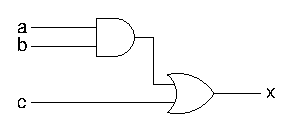
\includegraphics{../figures/xfig/andor.eps}
    \caption{Connecting output of \textit{and2} to input of $\mathit{or2}$}
    \label{fig:andor}
  \end{center}
\end{figure}

\section{Circuit Definitions}
\label{sec:circuit-definitions}

\begin{verbatim}
> mux1 :: Signal a => a -> a -> a -> a
> mux1 c x y = or2 (and2 (inv c) x) (and2 c y)
\end{verbatim}

\begin{verbatim}
> mux2 :: Signal a => (a,a) -> a -> a -> a -> a -> a
> mux2 (c,d) p q w r =
>   mux1 c (mux1 d p q) (mux1 d w r)
\end{verbatim}

\begin{verbatim}
> winv4 :: Signal a => [a] -> [a]
> winv4 [x0,x1,x2,x3]
>   = [inv x0, inv x1, inv x2, inv x3]
\end{verbatim}

\begin{verbatim}
> halfAdd :: Signal a => a -> a -> (a,a)
> halfAdd x y = (and2 x y, xor2 x y)
\end{verbatim}

\begin{verbatim}
> bsum, bcarry :: Signal a => (a,a) -> a -> a
> bsum (x,y) c = xor3 x y c
> bcarry (x,y) c = or3 (and2 x y) (and2 x c) (and2 y c)
\end{verbatim}

\begin{verbatim}
> fullAdd :: Signal a => (a,a) -> a -> (a,a)
> fullAdd (x,y) c = (bcarry (x,y) c, bsum (x,y) c)
\end{verbatim}

\begin{verbatim}
> rippleAdd4 :: Signal a => a -> [(a,a)] -> (a,[a])
> rippleAdd4 c [(x0,y0),(x1,y1),(x2,y2),(x3,y3)]
>   = (c0, [s0,s1,s2,s3])
>   where
>     (c0,s0) = fullAdd (x0,y0) c1
>     (c1,s1) = fullAdd (x1,y1) c2
>     (c2,s2) = fullAdd (x2,y2) c3
>     (c3,s3) = fullAdd (x3,y3) cin
\end{verbatim}

\begin{figure}[htbp]
  \begin{center}
    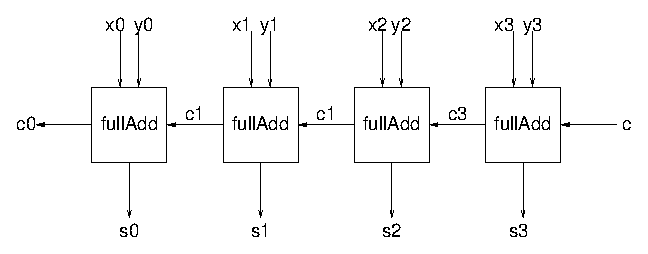
\includegraphics{../figures/xfig/rippleAdd4.eps}
    \caption{4-Bit Ripple Carry Adder}
    \label{fig:rippleAdd4}
  \end{center}
\end{figure}

\section{Equations}
\label{sec:equations}

See Figure \ref{fig:andor}.
\begin{verbatim}
x = or2 (and2 a b) c
\end{verbatim}

\section{Specification Modules}
\label{sec:spec-modules}

A Hydra file, like this one, begins with a statement that gives a name
to the module (this module is named Tutorial1).

\begin{verbatim}
module LogicGates where
\end{verbatim}

After the "module" statement there should be one or more "import"
statements saying which other library modules need to be loaded.  The
first line, "import Hydra", loads all the Hydra software tools, and
the second one, "import StdCircuit", loads the standard library of
circuits provided by Hydra.  There are many other combinations of
modules that can be imported, depending on what you want to do, but
usually it's most convenient to import just these two.

\begin{verbatim}
import Hydra
import CircuitLib
\end{verbatim}

Here's a definition of a new circuit, named `circ1'.

\begin{verbatim}
circ1 :: Signal a => a -> a -> a
circ1 x y = and2 (inv x) y
\end{verbatim}

It can be tested by checking its truth table:

\begin{verbatim}
truthTable21 circ1
\end{verbatim}

Commands begin with :, and :l says to load a file (you can also write
it as :load).  The Haskell interpreter will load various Hydra files,
and then give another prompt, which should look like

\begin{verbatim}
Tutorial1> 
\end{verbatim}

This means you can do simulations using all the definitions contained
in this file, as well as the standard Hydra definitions (those are
available because of the import statements near the beginning of this
file).

\chapter{Circuit Types}
\label{sec:circuit-types}

A specification consists of two parts: (1) the type specification,
which is optional, and (2) the behaviour specification, which is
required.  For example, the first line of the following specification
gives the type of circ and the second defines its internal structure:
\begin{verbatim}
circ :: Signal a => a -> a
circ x = inv x
\end{verbatim}

\section{Semantic Models and Signal Classes}
\label{sec:models-classes}

\subsection{Combinational Circuits}
\label{sec:combinational-circuits}

\subsection{Sequential Circuits}
\label{sec:sequential-circuits-1}

\subsection{Feedback}
\label{sec:feedback}

\begin{verbatim}
> reg1 :: Clocked a => a -> a -> a
> reg1 ld x = r
>   where r = dff (mux1 ld r x)
\end{verbatim}

\begin{figure}[htbp]
  \begin{center}
    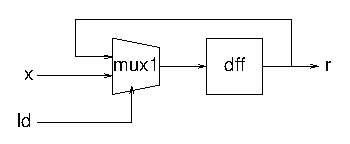
\includegraphics{../figures/xfig/reg1.eps}
    \caption{Register Bit}
    \label{fig:reg1}
  \end{center}
\end{figure}

\begin{verbatim}
> reg4 :: Clocked a => a -> [a] -> [a]
> reg4 ld [x0,x1,x2,x3] =
>   [reg1 ld x0, reg1 ld x1, reg1 ld x2, reg1 ld x3]
\end{verbatim}

\section{Grouped Signals}
\label{sec:grouped-signals}

Circuits often contain groups of signals that belong together.  In the
physically fabricated circuit the signals correspond to completely
independent wires, but the designer may prefer to think of them more
abstractly as a single value, such as a binary number.

One of the benefits of a hardware description language is the ability
to give a name to a group of signals and to treat it as a single
entity.  This reduces the number of named objects that the designer
has to keep in mind, and it allows circuits to be specified more
concisely.

There are a number of operations that can be applied to tuples and
words, such as extracting individual signals from a group.  It is
important to remember that operations on signal groups are purely
notational techniques, but they do not correspond to actualy
components in a circuit.

Hydra provides two mechanisms for grouping signals together: tuples
and words.  This section introduces both of these, and then shows how
they are used to simplify circuit specifications.

\subsection{Tuples}
\label{sec:tuples}

Tuples are used to group together signals that are related to each
other, but which do not represent the bits in a number.  The syntax
for tuples requires the signals to be separated by commas, and the
entire tuple is surrounded by parentheses (round brackets).  For
example, if $a$ and $b$ are signals, then $(a,b)$ is a tuple
containing them both.

A tuple may have any number of components.  Thus $(a,b)$ is a 2-tuple,
or pair, $(a,b,c)$ is a 3-tuple or triple, and so on.  A tuple cannot
have just one element; if you write $(a)$ this means just the signal
$a$.  This is because anything written in parentheses \emph{without}
commas inside is just an expression.  However, the empty 0-tuple $()$,
which is a group containing no signals, is allowed, though seldom
used.

There are two ways to give a name to a tuple: equations and formal
argument bindings.

(a,b)

(w,x,y,z)

ctl = (w,x,y,z)

\subsection{Words}
\label{sec:words}

Indexing !!

Concatenation ++

head, tail

Attaching an element :

Pattern matching [a,b,c]

Pattern matching :

\begin{verbatim}
lsb, msb :: [a] -> a
\end{verbatim}

Shift a word to the right (shr) or to the left (shl).  In both
cases, this is just a wiring pattern.  A 0 is brought in on one
side, and the bit on the other side is just thrown away.

\begin{verbatim}
> shr x = zero : [x!!i | i <- [0..k-2]]
>   where k = length x
> shl x = [x!!i | i <- [1..k-1]] ++ [zero]
>   where k = length x
\end{verbatim}

\section{Input and Output Ports}
\label{sec:input-output-ports}

\subsection{Port Specifications}
\label{sec:port-specifications}

\subsection{Multiple Inputs}
\label{sec:multiple-inputs}

\subsection{Multiple Outputs}
\label{sec:multiple-outputs}

\subsection{Fanout and Partial Applications}
\label{sec:fanout-part-appl}

Suppose you have a circuit $f$ that takes two inputs, an opcode
\textit{op} and a data input $x$.  Often one needs to apply such a
circuit to every bit in a word, but where each bit position receives
the same opcode.  That is, given input $[x_0, x_1, \ldots, x_{k-1}]$,
we want the output to be \[[f op x_0, f op x_1, \ldots, f op
x_{k-1}.\]

One way to express this is by writing out all the applications
explicitly:
\begin{verbatim}
circ_v1 op [x0,x1,x2,x3] =
  [f op x0, f op x1, f op x2, f op x3]
\end{verbatim}
A more concise way to write it is to define locally a special version
of $f$ that is already connected to the shared signal \textit{op}.
Calling this specialized circuit $g$, we have a second version of the
circuit:
\begin{verbatim}
circ_v2 op [x0,x1,x2,x3] = [g x0, g x1, g x2, g x3]
  where g x = f op x
\end{verbatim}
It is straightforward to see that the two circuits are equivalent.
For the first bit position, we can use the definition of g to
calculate $g x0 = f op x0$.  An equivalent way to write this
definition is to omit that last $x$ on both sides of the equation
defining $g$, leading to a third version:
\begin{verbatim}
circ_v3 op [x0,x1,x2,x3] = [g x0, g x1, g x2, g x3]
  where g = f op
\end{verbatim}
The choice between versions 2 and 3 is entirely stylistic; it's just a
matter of personal taste.  Version 2 may seem more straightforward at
first, but version 3 is more concise, as it allows you to define the
specialized circuit just by writing $(f\ \mathit{op})$ as an
expression, without even requiring an equation.

A definition like $g$ is called a \textit{partial application},
because it is an $f$ box applied to a partial set of its inputs, but
not all of them.  Partial applications are frequently useful in
conjunction with design patterns.  For example, we could generalize
the circuit defined above to work on words of arbitrary size using a
\textit{map} pattern, as follows:
\begin{verbatim}
circ op xs = map (f op) xs
\end{verbatim}
Note that we cannot write $\mathit{map2}\ f\ \mathit{op}\ \mathit{xs}$
because \textit{op} is not a word.  For another example of the use of
partial applications, see the shift register definitions in Section
??.

\begin{verbatim}
circ :: Signal a => a -> a -> (a,a)
circ a b = (y,z)
  where
    p = inv a
    y = and2 p b
    z = or2 p b
\end{verbatim}


\chapter{A Library of Circuits}
\label{cha:library-circuits}



\section{Bit level circuits}
\label{sec:bit-level-circuits}

This section describes the circuits that operate on individual bits,
including basic logic gates and basic building blocks.

The name `a' is the bit signal type (for example, Bool).



\subsection{Constant signal values}
\label{sec:const-sign-valu}

These constant values are defined for all signal types.

\begin{tabular}[c]{lll}
Component & Type & Description \\
zero & $a$ & Constant signal 0 \\
one  & $a$ & Constant signal 1
\end{tabular}


\subsection{Logic gates}
\label{sec:logic-gates-1}

These components are defined for all signal types.

\begin{tabular}[c]{|lll|}
\hline
Component & Type & Description \\
\hline
buf & $a \rightarrow a$
  & Buffer: amplifies signal but doesn't change it \\
inv & $a \rightarrow a$
  & Inverter: logical negation of input \\
and2 & $a \rightarrow a \rightarrow a$
  & 2-input logical and gate \\
nand2 & $a \rightarrow a \rightarrow a$
  & 2-input logical not-and gate \\
or2 & $a \rightarrow a \rightarrow a$
  & 2-input logical inclusive or gate \\
xor2 & $a \rightarrow a \rightarrow a$
  & 2-input logical exclusive or gate \\
nor2 & $a \rightarrow a \rightarrow a$
  & 2-input logical not-or gate \\
xnor2 & $a \rightarrow a \rightarrow a$
  & 2-input logical exclusive not-or gate \\
and3 & $a \rightarrow a \rightarrow a \rightarrow a$
  & 3-input logical and gate \\
nand3 & $a \rightarrow a \rightarrow a \rightarrow a$
  & 3-input logical not-and gate \\
or3 & $a \rightarrow a \rightarrow a \rightarrow a$
  & 3-input logical inclusive or gate \\
xor3 & $a \rightarrow a \rightarrow a \rightarrow a$
  & 3-input logical exclusive or gate \\
nor3 & $a \rightarrow a \rightarrow a \rightarrow a$
  & 3-input logical not-or gate \\
xnor3 & $a \rightarrow a \rightarrow a \rightarrow a$
  & 3-input logical exclusive not-or gate \\
and4 & $a \rightarrow a \rightarrow a \rightarrow a$
  & 4-input logical and gate \\
nand4 & $a \rightarrow a \rightarrow a \rightarrow a$
  & 4-input logical not-and gate \\
or4 & $a \rightarrow a \rightarrow a \rightarrow a$
  & 4-input logical inclusive or gate \\
xor4 & $a \rightarrow a \rightarrow a \rightarrow a$
  & 4-input logical exclusive or gate \\
nor4 & $a \rightarrow a \rightarrow a \rightarrow a$
  & 4-input logical not-or gate \\
xnor4 & $a \rightarrow a \rightarrow a \rightarrow a$
  & 4-input logical exclusive not-or gate \\
\hline
\end{tabular}


\subsection{Basic combinational circuits}
\label{sec:basic-comb-circ}

\begin{itemize}
  
\item $\mathit{winv4}\ ::\ \mathit{Signal}\ a \Rightarrow [a]
  \rightarrow [a]$ \hfill\break $ys = inv4 xs$ \hfill\break A 4-bit
  word inverter.  The input \textit{xs} is a word $[x_0,x_1,x_2,x_3]$
  of signals, which must have four elements, and the output word
  \textit{ys} is the bitwise inversion of \textit{xs}.

\item $\textit{rippleAdd4}\ ::\ \textit{Signal}\ a\ \Rightarrow
     a \rightarrow [(a,a)] \rightarrow (a,[a]) $ \hfill\break
  Example: $(c',s)\ =\ \textit{rippleAdd4}\ c\ \textit{z}$ \hfill\break
  Example: $(c',[s_0, s_1, s_2, s_3)\ =\ \textit{rippleAdd4}\ c
    \ [(x_0,y_0), (x_1,y_1), (x_2,y_2), (x_3,y_3)]$ \hfill\break
  A 4-bit ripple carry adder.  The sum of the carry input $c$ and two
  four-bit words $x = [x_0, x_1, x_2, x_3]$ and $y = [y_0, y_1, y_2, y_3]$
  which are input in bit slice format.  The output consists of a carry
  output c' and a sum word $s = [s_0, s_1, s_2, s_3]$.  The circuit
  satisfies the specification
     \[\textit{bin}\ (c':s)\ =\ \textit{bin}\ x\ +\ \textit{bin}\ y\ 
     +\ \textit{bit}\ c\]

\end{itemize}

\chapter{Simulation}
\label{sec:simulation}

A circuit can be tested by fabricating it from physical electronic
devices, providing it with suitable input signals, and checking that
the output signals are correct.  Ultimately, this is the only way to
test hardware fully, but it is often more effective to use simulation
during the design process.

A circuit simulator is a program that reads in the values of the input
signals to a circuit, and predicts the outputs which the circuit would
produce.  A circuit simulator will not account for all possible
phenomina in the real circuit.  For example, a logic simulator will
model the signals as Boolean values, but will ignore electrical issues
such as capacitance.

Simulation allows for testing during development, and it speeds up
debugging a design since it's quicker to rerun a simulation than to
refabricate the hardware every time a modification is made to the
design.  Simulation is analogous to software testing. For complex
circuits it is infeasible to simulate using all possible inputs, it is
important to pick good test inputs in order to find as many problems
as possible.  Simulation tests cannot establish the correctness of a
circuit---only formal methods can do that---but they often provide the
fastest method for eliminating errors.  Simulation and formal
correctness proofs are complementary methods, and both are useful in
producing correct, robust designs.

\section{Combinational Logic Simulation}
\label{sec:combinational-logic-simulation}

A combinational circuit has no state; it computes a pure logic
function.  A circuit is combinational if it contains only logic gates
(no flip flops), and there are no feedback loops within the circuit.

In this section we consider only logic simulation using the Boolean
signal class \textit{SigBool}.  It is also possible to simulate
combinational circuits using a multi-value logic, allowing CMOS
circuits to be handled, and to use a semantic model that keeps track
of gate delays, allowing hazards to be analysed.

\subsection{Applying a Circuit to its Inputs}
\label{sec:applying-circuit-inputs}

Since a circuit is modelled as a function, you can simulate it simply
by applying the function to suitable inputs.  This method is useful
for quick experiments on simple circuits using the Boolean model,
where the signal values are either \textit{True} or \textit{False}.

To simulate logic gates, first load the \textit{SigBool} module:
\begin{verbatim}
:load SigBool
\end{verbatim}
Now the inverter can be tested by entering the expresions
$\mathit{inv}\ \textit{True}$ and $\mathit{inv}\ \mathit{False}$ at
the interactive prompt.  This produces the following result:
\begin{verbatim}
*SigBool> inv True
False
*SigBool> inv False
True
\end{verbatim}
It's also possible to simulate simple circuits directly:
\begin{verbatim}
*SigBool> and2 True (or2 False True)
True
*SigBool> and2 False (or2 False True)
False
\end{verbatim}

Normally it's easier to define a module containing a circuit
definition, using named signals.  For example, you can save the
following text in a file named \texttt{Example1.hs} in your workspace
directory.  (The line \texttt{import CombTools} can be omitted now,
but we'll use it inthe next section.)
\begin{verbatim}
module Example1 where

import Signal
import SigBool
import CombTools

testcirc :: Signal a => a -> a -> a -> a
testcirc a b c = or2 (and2 a b) c
\end{verbatim}
Make sure you're in the workspace directory, enter Hydra, and load the
module:
\begin{verbatim}
:load Example1
\end{verbatim}
Now you can simulate the circuit on a variety of inputs:
\begin{verbatim}
*Example1> testcirc False True False
False
*Example1> testcirc False True True 
True
\end{verbatim}

%\begin{exercise}
%Simulate the value of \texttt{and3 False True True}.
%\end{exercise}

%\begin{exercise}
%Problem 1a.  Enter the following expression:
%truthTable31 circuit1a
%\begin{verbatim}
%> circuit1a a b c = inv (xor2 (and2 a b) (or2 b c))
%\end{verbatim}
%\end{exercise}

\subsection{Generating Truth Tables}
\label{sec:generate-truth-table}

Truth tables are a good way to describe the behaviour of combinational
circuits, as long as they don't have too many inputs.  Truth tables
can be used in two ways.  This section shows how to test an existing
circuit by generating its truth table; in effect, this is simulating
the circuit on all possible inputs.  Section ?? shows how Hydra can
automatically synthesise a circuit given an abstract specification of
its behaviour.

Hydra provides a family of tools for generating truth tables for
combinational circuits.  For example, the \textit{truthTable11}
function takes a combinational circuit with 1 input and 1 output, and
prints its truth table.
\begin{verbatim}
truthTable11 inv
truthTable11 buf
\end{verbatim}
There are similar functions for circuits with $i$ inputs and $j$
outputs, for $i \leq 4$ and $j\leq2$.  You can generate the truth
tables for various logic gates by entering expressions like the
following:
\begin{verbatim}
truthTable21 or2
truthTable31 nand3
truthTable41 xor4
truthTable22 halfAdd
truthTable22 demux1
\end{verbatim}

If a circuit takes an input word and produces an output word, then its
truth table can be generated using the \textit{truthTable} function.
This takes two arguments: the size $k$ of the input word, and the
circuit.  For example, we can define a circuit \textit{inv4} that
inverts a 4-bit word:
\begin{verbatim}
> winv4 :: Signal a => [a] -> [a]
> winv4 [x0,x1,x2,x3]
>   = [inv x0, inv x1, inv x2, inv x3]
\end{verbatim}
Now its truth table can be generated by entering
\begin{verbatim}
truthTable 4 winv4
\end{verbatim}

Many circuits cannot be handled directly using either
\textit{truthTable} or the \textit{truthTableij} family.  These
include circuits with too many inputs or outputs, and ones that have
signals with special grouping.  It is still straightforward to
generate their truth tables; you just need to make a temporary
definition of an equivalent circuit with the inputs all in one word,
and the outputs all in another.  For example, the full adder circuit
(module \textit{BitComb}) has type
\begin{equation}
  \label{eq:3}
  \mathit{fullAdd}\ ::\ \mathit{Signal}\ a\ \Rightarrow\
    (a,a) \rightarrow a \rightarrow (a,a)
\end{equation}
Even though this has only 3 inputs and 2 outputs, we can't use
\textit{truthTable32} because the first two inputs are grouped in a
tuple.  However, we can test it by using a \textbf{let} expression to
define an equivalent circuit \textit{f} which is compatible with
\textit{truthTable}:
\begin{verbatim}
>      let f [x,y,c] =
>            let (c',s) = fullAdd (x,y) c
>              in [c',s]
>        in truthTable 3 f
\end{verbatim}

\begin{exercise}
Produce a truth table for the \texttt{xor3} logic gate.
\end{exercise}

\begin{exercise}
  Produce a truth table for the 4-bit ripple carry adder,
  \textit{rippleAdd4}.  Choose randomly a few of the lines of this
  rather lengthy table, and verify that the circuit's outputs are
  correct.
\end{exercise}

\begin{exercise}
Problem 1b.  Enter the following expression:
truthTable31 circuit1b
\begin{verbatim}
> circuit1b x y z =
>   let a = and3 x y z
>       b = or2 y z
>   in (a, xor2 a b)
\end{verbatim}
\end{exercise}

\subsection{Number System Conversions}
\label{sec:number-sys-conversion}

There are functions for converting between natural numbers (using
binary representation), integers (using two's complement
representation) bit strings, and hexadecimal.

The functions most useful for generating input signals are: intbit
intbin inttc hexbin hextc.

The functions most useful for interpreting output signals are: bitint
binint tcint binhex tchex.

\textit{more later...}

\section{Sequential Simulation}
\label{sec:sequential-simulation}

Circuits often have large numbers of input and output signals. It can
be difficult and error prone to set up the inputs for a simulation, as
well as to interrpret the outputs.  For example, it is straightforward
but tedious to convert decimal numbers to binary or two's complement
representations.  Furthermore, an actual simulation requires the
inputs to be expressed in a signal class instance.  This is
essentially a data structure intended for internal use only, and the
circuit designer should not need to delve into Hydra's internal data
structures.

solution: a software interface to the simulation, called a simulation
driver. It allows input to be provided in a readable form, and
translates this to the actual signal inputs required by the
circuit. Conversely, it takes the cirucuit's output signals, converts
them to a convenient notation, and formats them neatly for output.

It's important to be clear about what is software and what is
hardware--especially when the hardware isn't really hard, but is
actually being created virtually via simulation!

Formatting input and output signals

A "simulation driver" is a piece of software that takes input in a
readable form, runs the simulation, and formats the output signals.
We will use a simulation driver for each of our main circuits. 
We'll provide inputs to sequential circuits by making a list, where
each line of the list corresponds to a clock cycle, and it contains
the input signal values for that cycle (expressed in decimal).

\subsection{Providing Input to a Circuit}
\label{sec:providing-input}

The inputs for a simulation are written as lists of integers, and the
simulation driver contains format specifiers that say how to obtain
the signals from these integers.

The simulation input is a value of type $[[\textit{Int}]]$, and is
typically given the name \textit{input}.  The $i$th element of
\textit{input} specifies all the circuit inputs for clock cycle $i$,
and is a list of elements that define the input signal values during
cycle $i$.

Each clock cycle input is a list of integers.  The signals are
calculated from those integers using \emph{input format specifiers.}
Generally, each signal comes from one element of the list.  Each
signal is defined by an equation of the form
\begin{equation}
  \label{eq:1}
  \mathit{signal}\ =\ \mathit{format}\ \mathit{input}\ i
\end{equation}
where $i$ is an index within the list of integers for the cycle.  For
example, the equation
\begin{equation}
  \label{eq:2}
  x\ =\ \mathit{getbit}\ \mathit{input}\ 3
\end{equation}
says that the signal $x$ is a bit whose value is given in the third
element of \textit{input}.

A variety of input formats are provided, allowing you to extract bits
and words, using either binary or two's complement representation.
The most frequently used input formats are:

\begin{itemize}
\item $b\ =\ \mathit{getbit}\ \mathit{input}\ i$ defines $b$ as a bit
  signal representing the $i$th element of the input list.  The value
  of $b$ during a clock cycle is \textit{zero} if the corresponding
  input integer is 0, and \textit{one} if the integer is 1.
\item $w\ =\ \mathit{getbin}\ k\ \mathit{input}\ i$ defines $w$ to be
  a $k$-bit word whose binary interpretation is the $i$th integer in
  the input list.
\item $w\ =\ \mathit{gettc}\ k\ \mathit{input}\ i$ defines $w$ to be a
  $k$-bit word whose two's complement interpretation is the $i$th
  integer in the input list.
\end{itemize}

\subsection{Interpreting the Output from a Circuit}
\label{sec:interpr-outp-from}

The output signals produced by a circuit may be hard to read directly,
partly because there are likely to be too many bits to grasp easily,
and partly because the data structures that Hydra uses to represent
clocked signals contain a lot of detail.

To make the outputs more readable, a simulation driver uses a format
specification to construct neat textual output.  A complete format is
a list of individual specifiers, each of which produces one or more
characters of output. The output specification can be given a name
like \textit{simoutput}, and defined as follows
\begin{align*}
  & \mathit{simoutput}\ ::\ [\mathit{Format}\ \mathit{Bool}] \\
  & \mathit{simoutput}\ =\ [\ldots\ \textit{list of format specifiers}\ \ldots]
\end{align*}

The format specifiers are:

\begin{itemize}
\item $\mathit{bit}\ b$ outputs the bit $b$ in one character, which
  will be either \texttt{0} or \texttt{1}.
\item $\mathit{bits}\ w$ outputs the word $w$ in a string of length
  $k$ consisting of \texttt{0}s and \texttt{1}s, where $k$ is the size
  of $w$.
\item $\mathit{hex}\ w$ outputs the word $w$ as a hexadecimal string.
  The size of the string is the $\lceil k/4 \rceil$ ($k/4$ rounded up
  to an integer), which is the minimal size needed to represent $w$.
\item $\mathit{bindec}\ k\ w$ interprets the word $w$ as a binary
  representation, and converts it to a decimal number $k$ characters
  wide.  Leading spaces are attached if necessary to fill the field.
\item $\mathit{tcdec}\ k\ w$ interprets the word $w$ as a two's
  complement representation, and converts it to a decimal number $k$
  characters wide.
\item $\mathit{string}\ s$ outputs the character string $s$, which is
  useful for labelling signals, inserting newlines, etc.
\end{itemize}

\subsection{Simulation Drivers}
\label{sec:simulation-drivers}


The simulation driver for a synchronous circuit contains four main
pieces:

\begin{itemize}
\item Definitions of the circuit parameters, if any; these typically
  include word size and address size.
\item An equation that applies the circuit to its inputs, defining
  names for the outputs.
\item Tools that take the inputs expressed in a form easy for the user
  to write and convert them to the proper input signal representation.
\item Tools that take the output signals from the circuit and format
  them readably.
\end{itemize}

The simulation is performed by executing the IO operation \textit{run
  input simoutput}, where $\textit{input} :: [[\textit{Int}]]$ is the
input data specified by the user.  Thus the form of a typical simulation
  driver is
\begin{align*}
  & \mathit{simoutput}\ ::\ [\mathit{Format}\ \mathit{Bool}] \\
  & \mathit{simoutput}\ =\ [\ldots\ \textit{list of format specifiers}\ \ldots]
\end{align*}

\subsection{Example: A Simple Simulation Driver}
\label{sec:example-sim-driver}

The tools for writing simulation drivers are illustrated in this
section by a simple standalone driver, which reads some signals and
then just outputs them directly, without processing them with a circuit.

In this experiment, there are three inputs: a bit $x$, an 8-bit binary
number $y$, and an 8-bit two's complement number $z$.  Each line of
the input will be specified with integers for $x$, $y$, ans $z$ in
order.  A particular input data set \textit{test\_input} is defined
below.  It's a good idea to line up the elements neatly, so that any
signal can be followed through time by reading down a column.
Comments are used to label each column with the signal name, and to
say what the representation for that signal is.  In this example, the
cycle numbers are labelled as well.  Normally this is unnecessary, but
in a test case that runs for only a few cycles it may be helpful.

\begin{verbatim}
> test_input :: [[Int]]
> test_input =
> --  x    y     z
> -- bit  bin   tc
> -- ~~~~~~~~~~~~~~~
>   [[0,    5,    5],     -- cycle 0
>    [1,  255,   -1],     -- cycle 1
>    [1,    0,  127],     -- cycle 2
>    [0,   42, -128],     -- cycle 3
>    [1,  195,  -37]      -- cycle 4
>   ]
\end{verbatim}

\begin{verbatim}
> standalone_driver :: [[Int]] -> IO ()
> standalone_driver input = do run input simoutput
>   where
>
> -- Size parameters
>     n = 8
>
> -- Input formatting
>     x = getbit   input 0 :: Stream Bool
>     y = getbin n input 1
>     z = gettc  n input 2
>
> -- Output formatting
>     simoutput :: [Format Bool]
>     simoutput =
>       [string "x = ", bit x,
>        string "      y = ", hex y, bindec 5 y, tcdec 5 y,
>        string "      z = ", hex z, string " ", bits z,
>          bindec 5 z, tcdec 5 z]
\end{verbatim}

The simulation can now be performed by running the driver with an
input data set.  One way is to enter the expression
\begin{verbatim}
standalone_driver test_input
\end{verbatim}
at the interactive prompt.  With larger design projects, it's useful
to define a batch script \texttt{main} which executes the test.  This
allows many test cases to be run together.  It is a good idea to run
such batch tests regularly as a design is developed, to ensure that
any changes haven't introduced bugs.
\begin{verbatim}
> main :: IO ()
> main =
>   do standalone_driver test_input
\end{verbatim}

The output from executing \texttt{main} is shown below.  From the
output it's easy to see that $x$ is the same values as were specified
in the input.  The second signal, $y$, is an 8-bit word which is
displayed three ways: as a hexadecimal, as an integer using binary
representation, and as an integer using two's complement
representation.  Note that $y$ was input using a binary format
specifier, and the binary output gives exactly the same values.
Naturally, the two's complement output for $y$ is different; for
example, the word consisting of all 1s represents 255 in binary but -1
in two's complement.  Since $z$ was input using a two's complement
format, the two's complement output column shows the same values,
while the binary output column may be different.

\begin{verbatim}
*FormatTest> main
   0.  x = 0      y = 05    5    5      z = 05 00000101    5    5
   1.  x = 1      y = ff  255   -1      z = ff 11111111  255   -1
   2.  x = 1      y = 00    0    0      z = 7f 01111111  127  127
   3.  x = 0      y = 2a   42   42      z = 80 10000000  128 -128
   4.  x = 1      y = c3  195  -61      z = db 11011011  219  -37
\end{verbatim}

\subsection{Batch Testing}
\label{sec:batch-testing}

This is a single operation that runs the various examples above as one
large batch.  You can run it by just launching Hydra, loading this
file, and entering "main" at the prompt.

\begin{verbatim}
main =
  do putStrLn "Hydra: running Tutorial1 batch"
     sim_adder rippleAdd 16 add_input1
     sim_sr4 sr4_input
     sim_regfile
     sim_regfile_dec
     sim_rtm
     sim_mult
     putStrLn "Examples1 finished"
\end{verbatim}


\chapter{Design Patterns}
\label{sec:design-patterns}

asdf




\section{Mapping}
\label{sec:mapping}




\subsection{General map}
\label{sec:general-map}


\begin{verbatim}
map :: (a->b) -> [a] -> [b]
\end{verbatim}

\begin{verbatim}
> winv :: Signal a => [a] -> [a]
> winv x = map inv x
\end{verbatim}


\begin{verbatim}
> map2 :: (a->b->c) -> [a] -> [b] -> [c]
\end{verbatim}

\subsection{Explicitly Sized Map}
\label{sec:explicitly-sized-map}

\begin{verbatim}
> mapn :: (a->b) -> Int -> [a] -> [b]
\end{verbatim}

\begin{verbatim}
> reg :: Clocked a => Int -> a -> [a] -> [a]
> reg n ld x = mapn (reg1 ld) n x
\end{verbatim}

\begin{verbatim}
> mux1w :: Signal a => a -> [a] -> [a] -> [a]
> mux1w c x y = map2 (mux1 c) x y
\end{verbatim}

\subsection{Bit Slice Organization}
\label{sec:bit-slice-org}

\begin{verbatim}
> bitslice2 :: [a] -> [a] -> [(a,a)]
> bitslice2 = zip
\end{verbatim}

\begin{verbatim}
> unbitslice2 :: [(a,b)] -> ([a],[b])
> unbitslice2 [] = ([],[])
> unbitslice2 ((x,y):zs) =
>   let (xs,ys) = unbitslice2 zs
>   in (x:xs, y:ys)
\end{verbatim}

\begin{verbatim}
> zipn :: Int -> [a] -> [b] -> [(a,b)]
> zipn n x y =
>   [(x!!i,y!!i) | i <- [0..n-1]]
\end{verbatim}

\begin{verbatim}
> unzipn n xs =
>   ([fst (xs!!i) | i <- [0..n-1]],
>    [snd (xs!!i) | i <- [0..n-1]])
\end{verbatim}

\section{Linear Folding}
\label{sec:linear-folding}

\begin{verbatim}
foldr :: (b->a->a) -> a -> [b] -> a
foldr f a [] = a
foldr f a (x:xs) = f x (foldr f a xs)
\end{verbatim}

Binary comparitor
%~~~~~~~~~~~~~~~~~

\begin{verbatim}
> cmp1 :: Signal a => (a,a,a) -> (a,a) -> (a,a,a)
> cmp1 (lt,eq,gt) (x,y) =
>   (or2 lt (and3 eq (inv x) y),
>    and2 eq (inv (xor2 x y)),
>    or2 gt (and3 eq x (inv y))
>   )
\end{verbatim}

\begin{verbatim}
> rippleCmp :: Signal a => [(a,a)] -> (a,a,a)
> rippleCmp = foldl cmp1 (zero,one,zero)
\end{verbatim}

\section{Linear Scanning}
\label{sec:linear-scanning}

\begin{verbatim}
> wscanr :: (b->a->a) -> a -> [b] -> [a]
> wscanr f a xs =
>   [foldr f a (drop (i+1) xs) | i <- [0 .. length xs -1]]
\end{verbatim}

\begin{verbatim}
> ascanr ::  (b->a->a) -> a -> [b] -> (a,[a])
> ascanr f a [] = (a,[])
> ascanr f a (x:xs) =
>   let (a',xs') = ascanr f a xs
>       a'' = f x a'
>   in (a'', a':xs')
\end{verbatim}

\subsection{Inclusive Scans}
\label{sec:inclusive-scans}

\subsection{Mapping Scans}
\label{sec:mapping-scans}


\subsection{Bidirectional Scans}
\label{sec:bidirectional-scans}

Shift register

\begin{verbatim}
> sr :: (Signal a, Clocked a)
>   => (a,a) -> a -> a -> [a] -> (a,a,[a])
> sr op l r xs = mscan (srb' op) l r xs
>   where srb' a b c d = fanout3 (srb a b c d)
\end{verbatim}

\section{Tree Patterns}
\label{sec:tree-patterns}

\subsection{Tree Expansion: Downsweep}
\label{sec:tree-expansion}

\subsection{Tree Reduction: Upsweep}
\label{sec:tree-reduction}

And/Or over a word

Determine whether there exists a 1 in a word, or whether all the
bits are 0.  A tree fold can do this in log time, but for
simplicity this is just a linear time fold.

\begin{verbatim}
> any1, all0 :: Signal a => [a] -> a
> any1 = foldl or2 zero
> all0 = foldl and2 one
\end{verbatim}

\begin{verbatim}
> orw :: Signal a => [a] -> a
> orw = foldl or2 zero
\end{verbatim}

\subsection{Bidirectional Tree Sweep}
\label{sec:bidir-tree-sweep}

\section{Explicit Recursion}
\label{sec:explicit-recursion}


See Section \ref{sec:register-file}, which uses a recursive pattern to
define the register file circuit.

\chapter{Combinational Design}
\label{sec:combinational-design}

\section{Fanout}
\label{sec:fanout}

While designing combinational circuits, it is often necessary to make
one or more duplicate copies of a signal $x$.  This is called
\textit{fanout}, because a wire splits and ``fans out'' to several
destinations.

Fanout can be specified implicitly simply by using a signal in several
places.  For example, in the following definition the signal $x$ is
defined in one place, but used in several places, so the wire carrying
$x$ must fan out to each of the points where it is used.
\begin{verbatim}
circ a = ...
  where x = ...
        y = ... x ...
        z = ... x ...
\end{verbatim}
The fanout is implicit because the specification does not directly
mention it.

Sometimes it is better to specify fanout explicitly.  There are many
reasons for this.  Excessive fanout may cause delays or capacitance
problems in the circuit.  Since these issues belong at the electronic
level of abstraction, they are not apparent when simulating a circuit
at the logical level.  Such problems can be controlled by specifying
fanout explicitly.  Furthermore, fanouts must sometimes be requested
explicitly in order to use a design pattern.

The following circuits take a signal $x$ and fan it out into a tuple
containing several copies of $x$.  These circuits are pure wiring
patterns; they contain no logic gates.

\begin{verbatim}
> fanout2 :: a -> (a,a)
> fanout2 x = (x,x)

> fanout3 :: a -> (a,a,a)
> fanout3 x = (x,x,x)

> fanout4 :: a -> (a,a,a,a)
> fanout4 x = (x,x,x,x)
\end{verbatim}

When it is important to limit the degree of fanout, in order to avoid
problems at the electronic level, it is better to use buffered
fanouts.  These circuits are similar to the wiring patterns above, but
they use a buffer logic gate to bring the signal $x$ up to full
strength.

\begin{verbatim}
> fanoutbuf2 :: Signal a => a -> (a,a)
> fanoutbuf2 x = (y,y)
>   where y = buf x

> fanoutbuf3 :: Signal a => a -> (a,a,a)
> fanoutbuf2 x = (y,y,y)
>   where y = buf x

> fanoutbuf4 :: Signal a => a -> (a,a,a,a)
> fanoutbuf2 x = (y,y,y,y)
>   where y = buf x
\end{verbatim}

The next problem is to generalise fanout, so that a bit $x$ is
duplicated in order to form a $k$-bit word, for arbitrary $k$.  This
is performed by the \textit{fanout} circuit, which is a pure wiring
pattern, and \textit{fanoutbuf}, which uses buffered fanouts.
Normally it is better to use \textit{fanoutbuf}.

\begin{verbatim}
> fanout, fanoutbuf :: Signal a => Int -> a -> [a]
\end{verbatim}

For example, $\mathit{fanoutbuf}\ 6\ x$ produces a word whose value is
$[x,x,x,x]$, but it introduces buffers as needed to prevent any logic
gate from having to drive too many wires.

In RISC processors, the Boolean result $x$ of a comparison is usually
represented as an integer, where False is represented by 0 and True is
represented by 1.  In both cases, these will be $k$-bit binary
integers, so the rightmost bit should be the Boolean $x$, while all
the leading bits should be 0.  This task is performed by the
\textit{boolword} circuit, which uses a buffered fanout to produce the
leading zeros.

\begin{verbatim}
> boolword :: Signal a => Int -> a -> [a]
> boolword n x = fanoutbuf (n-1) zero ++ [x]
\end{verbatim}

\section{Multiplexers and Demultiplexers}
\label{sec:mux-demux}

\begin{verbatim}
> demux1 :: Signal a => a -> a -> (a,a)
> demux1 c x = (and2 (inv c) x, and2 c x)
\end{verbatim}

\begin{verbatim}
> mux22 :: Signal a => (a,a) -> (a,a) -> (a,a)
>            -> (a,a) -> (a,a) -> (a,a)
> mux22 (a,b) (w0,w1) (x0,x1) (y0,y1) (z0,z1) =
>   (mux2 (a,b) w0 x0 y0 z0,
>    mux2 (a,b) w1 x1 y1 z1)
\end{verbatim}

\section{Ripple Carry Adder}
\label{sec:ripple-carry-adder}

\subsection{Specification}
\label{sec:adder-specification}

\subsection{Implementation}
\label{sec:adder-implementation}

\subsection{Simulation}
\label{sec:adder-simulation}

Although the adder is a combinational circuit, it's easiest to test it
with a full-blown simulation driver that provides separate numbers to
add during each clock cycle.  Unless the wordsize is very small, the
adder has too many inputs for a truth table to be reasonable, and the
only way to test it is by providing a small subset of all the possible
inputs.  A simulation driver provides a systematic way to run a series
of tests over a sequence of clock cycles.

The simulation driver for and adder should let you write the input and
read the output in decimal notation.  There are three values to be
supplied for each clock cycle: the carry input $c$, and the two
numbers $x$ and $y$.  For each test case, the inputs will be written
as a list of three decimal numbersThese will be written in a list of
the form $[c, x, y]$.  The entire simulation input will be a list of
test cases which will be run in a succession of clock cycles.  An
example of the input is \textit{add\_input1}.

\begin{verbatim}
> add_input1 :: [[Int]]

> add_input1 =
> --  c   x    y
> -- bit bin  bin
> -- ~~~~~~~~~~~~~
>   [[0,   2,   3],
>    [0,   1,   8],
>    [0,  10,   5],
>    [0,  11,   2],
>    [1,   4,   5]]
\end{verbatim}

An important point to notice is that a simulation driver is concerned
only with the \emph{type} of a circuit, not with its internal
structure.  This means that we could have a variety of different
circuits that implement the same specification, an that share the same
type.  It's a good idea to exploit this by generalising the simulation
driver, so that it takes a particular circuit implementation as an
argument.  If we go on to optimise the circuit, in order to make it
faster, the same driver (and the same input) can be used to test each
version.  The adder simulation driver will work for any circuit that
has the appropriate type.  Since simulation drivers operate through a
sequence of clock cycles, they require the synchronous model to be
used. This means that the signal type $a$ must be in the
\textit{Clocked} class.
\begin{verbatim}
Clocked a => a -> [(a,a)] -> (a,[a])
\end{verbatim}
Since the ripple carry adder is a combinational circuit, it works with
all semantic models, so it has the more general type:
\begin{verbatim}
Signal a => a -> [(a,a)] -> (a,[a])
\end{verbatim}
Since any clocked signal is a signal, there is no problem with doing a
synchronous simulation of a combinational circuit.

The simulation driver is called \textit{sim\_adder}, and it takes
three arguments: the adder circuit to be tested, its wordsize, and the
input data.  For example, in order to test the 4-bit ripple carry
adder with the input data above, you can enter the following
expression at the interactive prompt:

\begin{verbatim}
sim_adder rippleAdd4 4 add_input1
\end{verbatim}

The simulation produces the following output:

\begin{verbatim}
WordCombTest> sim_adder rippleAdd4 4 add_input1

..................................................
   Simulating ripple carry adder
      0.   ci=0 x=   2 y=   3   Output: 0   5
      1.   ci=0 x=   1 y=   8   Output: 0   9
      2.   ci=0 x=  10 y=   5   Output: 0  15
      3.   ci=0 x=  11 y=   2   Output: 0  13
      4.   ci=1 x=   4 y=   5   Output: 0  10
..................................................
\end{verbatim}

We can try similar experiments by using the general $n$-bit circuit
\textit{rippleAdd}, by varying the wordsize, and by using alternative
test data.  The following experiments can be entered interactively, or
they can be gathered together into a batch simulation file.

\begin{verbatim}
sim_adder rippleAdd4  4 add_input1
sim_adder rippleAdd   4 add_input1
sim_adder rippleAdd  16 add_input1
\end{verbatim}

\emph{Note:  see module WordCombTest}

The adder has one circuit parameter, its wordsize, since our ripple
carry adders may be defined using design patterns that work for
arbitrary size!  Here we use 8-bit words.

\begin{verbatim}
n = 8
\end{verbatim}

The heart of the simulation driver is an equation that uses the
circuit.  Here, we define the carry output co and the sum word s to be
the outputs of an adder with input words x and y; these are
represented in bit slice form as a single word z :: [(a,a)].

\begin{verbatim}
(co,s) = rippleAdd ci z
\end{verbatim}

The bit slice word z is formed by the bitslice2 wiring pattern:
\begin{verbatim}
z = bitslice2 x y
\end{verbatim}
We could also omit this equation, and write the circuit application as
\begin{verbatim}
(co,s) = rippleAdd ci (bitslice2 x y)
\end{verbatim}

The inputs to the circuit can be provided interactively, but sometimes
it's more convenient to define a set of inputs as a constant
definition in the simulation module.  This allows us to run a
simulation repeatedly, without having to keep typing the same inputs
over and over again.  That approach will be taken here; later we will
introduce tools that support interactive simulations.

Now we need to use the tools for converting the test input to the
correct signal representations:

\begin{verbatim}
ci = getbit   input 0 :: Stream Bool 
   x  = getbin n input 1
   y  = getbin n input 2
\end{verbatim}

The first equation says that ci is obtained from the 0'th column of
the test input, using a bit conversion (getbit).  The second equation
says that x comes from column 1 in the test input, and it's converted
using a binary conversion (getbin n), where n is the wordsize.  The
last equation converts y from column 2 of the input data.

The final step is to format the output.  First, we specify the
underlying signal representation that is being used:

\begin{verbatim}
simoutput :: [Format Bool]
\end{verbatim}

This is necessary, because Hydra supports a large number of signal
representations, and it needs to know which one to use here.

Now we define the simulation output by formatting the various signals
that should be printed.  The format consists of a list of fields
separated by commas.  For every clock cycle, Hydra will print a line
comprising all these fields.  The field format specifications are

  string "abc"  prints the literal string on each line
  bit x         prints the value of the bit signal x, as 0 or 1
  bindec k x    converts the binary word x to a 4-digit decimal integer
  tcdec k x     converts the two's complement word x to a 4-digit
                decimal integer

The following format prints the adder's inputs and outputs, along with
some labels:

\begin{verbatim}
simoutput =
      [bit ci,
       string " x= ", bindec 4 x, tcdec 4 x,
       string " y= ", bindec 4 y, tcdec 4 y,
       string " Output: ", bit co,
       string " sum= ", bindec 4 s, tcdec 4 s]
\end{verbatim}

Putting all the pieces together, here is the simulation driver for the
ripple carry adder:

Here is the complete definition of the simulation driver.

\begin{verbatim}
sim_adder add_circuit n input =
  let (co,s) = add_circuit ci (bitslice2 x y)
      ci = getbit   input 0
      x  = getbin n input 1
      y  = getbin n input 2
      simoutput :: [Format Bool]
      simoutput =
        [string " ci=", bit ci,
         string " x= ", bindec 3 x,
         string " y= ", bindec 3 y,
         string "   Output: ", bit co, bindec 4 s]
  in do putStrLn "\nSimulating ripple carry adder"
        run input simoutput
\end{verbatim}

\subsection{Subtraction}
\label{sec:subtraction}

Two's complement addition and subtraction

\begin{verbatim}
> addSub :: Signal a => a -> [(a,a)] -> (a,[a])
> addSub sub xy = rippleAdd sub (map f xy)
>   where f (x,y) = (x, xor2 sub y)
\end{verbatim}


\section{Binary Integer Comparison}
\label{sec:binary-integer-comparison}

\subsection{Simulation Driver for Comparitor}
\label{sec:sim-driver-comp}


The ripple comparitor for binary numbers can be simulated by entering
the following:

\begin{verbatim}
sim_comparitor rippleCmp 16 cmp_input1
\end{verbatim}

Here is some test data for the comparitor...

\begin{verbatim}
> cmp_input1 :: [[Int]]
> cmp_input1 =
>   [[2, 3],
>    [3, 2],
>    [3, 3],
>    [1, 8],
>    [8, 1],
>    [9, 9],
>    [0, 5],
>    [7, 5]]
\end{verbatim}

The simulation driver is similar to the adder driver.

\begin{verbatim}
> sim_comparitor circuit n input =
>   let (lt,eq,gt) = circuit (bitslice2 x y)
>       x = getbin n input 0
>       y = getbin n input 1
>       simoutput :: [Format Bool]
>       simoutput =
>         [string " x= ", bindec 4 x,
>          string "   y= ", bindec 4 y,
>          string "  (lt,eq,gt) = ",
>          bit lt, bit eq, bit gt]
>   in do putStrLn "\nSimulating comparitor"
>         run input simoutput
\end{verbatim}

\section{Design of an ALU}
\label{sec:design-ALU}

\chapter{Sequential Design}
\label{sec:sequential-design}

\section{Shift Registers}
\label{sec:shift-registers}

\begin{verbatim}
> sr4_v1 :: Clocked a => (a,a) -> a -> a -> [a] -> [a]
> sr4_v1 op l r [x0,x1,x2,x3] = [a,b,c,d]
>   where
>      a = srb op l b x0
>      b = srb op a c x1
>      c = srb op b d x2
>      d = srb op c r x3
\end{verbatim}

\begin{verbatim}
> sr4_v2 :: Clocked a => (a,a) -> a -> a -> [a] -> [a]
> sr4_v2 op l r [x0,x1,x2,x3] = [a,b,c,d]
>   where
>      (opa,opb,opc,opd) = fanout4 op
>      a = srb opa l b x0
>      b = srb opb a c x1
>      c = srb opc b d x2
>      d = srb opd c r x3
\end{verbatim}

\begin{verbatim}
> sr4_v3 :: Clocked a => (a,a) -> a -> a -> [a] -> [a]
> sr4_v3 op l r [x0,x1,x2,x3] = [a,b,c,d]
>   where
>      f = srb op
>      a = f l b x0
>      b = f a c x1
>      c = f b d x2
>      d = f c r x3
\end{verbatim}

\begin{itemize}
\item Design a general shift register as follows:
  \begin{itemize}
  \item There are $n$ bit positions, each with one bit of state.
  \item There is an $n$-bit word input $a = [a_0, \ldots, a_{n-1}]$.
  \item There are two data inputs $l$ and $r$; $l$ is the left input
    (it comes into the leftmost position $0$), and $r$ is the right
    input (it comes into the rightmost position $n-1$).
  \item There is a two-bit control input $[c_0,c_1]$.  For
    convenience, we will refer to the four possible values of the
    control input as 0, 1, 2, and 3.
  \item The circuit has three outputs: an $n$-bit word which is the
    contents of the $n$ states; the left output (which is the value of
    bit 0) and the right output (which is the value of bit $n-1$).
    Notice that Bit 0 actually appears twice in the output, once as
    $l'$ and again as the 0'th bit of the output word; similarly Bit
    $n-1$ appears twice, once as $r'$ and also as bit $n-1$ of the
    output.
  \item At each clock tick, the behaviour is as follows:
\begin{center}
  \begin{tabular}{|l|l|l|} \hline
    $c$  &  \emph{action} & \emph{behaviour} \\ \hline
    0  &  clear  & $x_i := 0$ for $0 \leq i < n$ \\
    1  &  load   & $x_i := a_i$ for $0 \leq i <n$ \\
    2  &  shift left &$x_i := x_{i+1}$ for $0 \leq i \leq n-2$,
            $x_{n-1} := r$  \\
    3  &  shift right &$x_i := x_{i-1}$ for $1 \leq i \leq n-1$,
            $x_0 := l$\\
    \hline
  \end{tabular}
\end{center}
\item \textbf{Hint:} \emph{Figure out what's going on in each bit
    position, and design a circuit---you could call it
    \texttt{srb}---that implements an arbitrary position in the
    circuit.  Then design the entire circuit as a row of shift
    register bits, connnected together in an appropriate way.  If you
    like, you may simply design a version of the circuit at a specific
    wordsize, say 4 bits, but the most elegant approach is to use a
    combinator.}
\end{itemize}
\end{itemize}

\begin{verbatim}
> srb :: Clocked a => (a,a) -> a -> a -> a -> a
> srb op l r x = y
>   where y = dff (mux2 op y x l r)
\end{verbatim}

\begin{verbatim}
> sr4 :: Clocked a => (a,a) -> a -> a -> [a] -> [a]
> sr4 op l r [x0,x1,x2,x3] = [a,b,c,d]
>   where
>      a = srb op l b x0
>      b = srb op a c x1
>      c = srb op b d x2
>      d = srb op c r x3
\end{verbatim}

We can define the shift register circuit more generally with the
mscanr combinator; note that in this simulation, we use the general
circuit "sr" rather than the restricted 4-bit sr4.  The test data
is identical to that used above, and you can check that the circuit
defined in this more general way has the same behaviour on this
test data.

\begin{verbatim}
sim_gen_sr_4 =
  let input =
--      op  l  r  x        op    produce  state
--      ~~~~~~~~~~~       ~~~~~~~~~~~~~~~~~~~~~
       [[1, 0, 0, 9],  -- load     1001    0000
        [0, 0, 0, 3],  -- nop      1001    1001
        [2, 1, 0, 4],  -- right 1  1100    1001
        [2, 0, 0, 2],  -- right 0  0110    1100
        [3, 0, 1, 7],  -- left  1  1101    0110
        [1, 0, 0, 5],  -- load     0101    1101
        [0, 0, 0, 0]]  -- nop      0101    0101
      op = getbit2  input 0
      l =  getbit   input 1
      r =  getbit   input 2
      x =  getbin 4 input 3
      (op0,op1) = op
      (p,q,y) = sr op l r x
      simoutput :: [Format Bool]
      simoutput = [string "Input: ",
              bit op0, bit op1, string " ",
              bit l, string " ", bit r, string " ", bits x,
              string "    Output: ",
              bit p, bit q, string " ", bits y]
  in do putStrLn "\nSimulate n-bit shift register, size 4"
        run input simoutput
\end{verbatim}

Here is a similar example, but where the word size is increased to
8.  Notice that all we had to do to change the wordsize was to
change the number of bits in x; the general mscanr combinator
automatically accommodates itself to the new word size!

\begin{verbatim}
sim_gen_sr_8 =
  let input =
--      op  l  r  x        op        state
--      ~~~~~~~~~~~       ~~~~~~~~~~~~~~~~~~~~~
       [[1, 0, 0, 75],  -- load     0000 0000
        [0, 0, 0,  3],  -- nop      0100 1011
        [2, 1, 0,  4],  -- right 1  0100 1011
        [2, 0, 0,  2],  -- right 0  1010 0101
        [3, 0, 1,  7],  -- left  1  0101 0010
        [1, 0, 0,  5],  -- load     1010 0101
        [0, 0, 0,  0]]  -- nop      0000 0101
      op = getbit2  input 0
      l =  getbit   input 1
      r =  getbit   input 2
      x =  getbin 8 input 3  -- 8 bit words!
      (op0,op1) = op
      (p,q,y) = sr op l r x
      simoutput :: [Format Bool]
      simoutput = [string "Input: ",
              bit op0, bit op1, string " ",
              bit l, string " ", bit r, string " ", bits x,
              string "    Output: ",
              bit p, bit q, string " ", bits y]
  in run input simoutput
\end{verbatim}

We can define the shift register circuit more generally with the
mscanr combinator; note that in this simulation, we use the general
circuit "sr" rather than the restricted 4-bit sr4.  The test data
is identical to that used above, and you can check that the circuit
defined in this more general way has the same behaviour on this
test data.

\begin{verbatim}
sim_gen_sr_4 =
  let input =
--      op  l  r  x        op    produce  state
--      ~~~~~~~~~~~       ~~~~~~~~~~~~~~~~~~~~~
       [[1, 0, 0, 9],  -- load     1001    0000
        [0, 0, 0, 3],  -- nop      1001    1001
        [2, 1, 0, 4],  -- right 1  1100    1001
        [2, 0, 0, 2],  -- right 0  0110    1100
        [3, 0, 1, 7],  -- left  1  1101    0110
        [1, 0, 0, 5],  -- load     0101    1101
        [0, 0, 0, 0]]  -- nop      0101    0101
      op = getbit2  input 0
      l =  getbit   input 1
      r =  getbit   input 2
      x =  getbin 4 input 3
      (op0,op1) = op
      (p,q,y) = sr op l r x
      simoutput :: [Format Bool]
      simoutput = [string "Input: ",
              bit op0, bit op1, string " ",
              bit l, string " ", bit r, string " ", bits x,
              string "    Output: ",
              bit p, bit q, string " ", bits y]
  in do putStrLn "\nSimulate n-bit shift register, size 4"
        run input simoutput
\end{verbatim}


Here is a similar example, but where the word size is increased to
8.  Notice that all we had to do to change the wordsize was to
change the number of bits in x; the general mscanr combinator
automatically accommodates itself to the new word size!

\begin{verbatim}
sim_gen_sr_8 =
  let input =
--      op  l  r  x        op        state
--      ~~~~~~~~~~~       ~~~~~~~~~~~~~~~~~~~~~
       [[1, 0, 0, 75],  -- load     0000 0000
        [0, 0, 0,  3],  -- nop      0100 1011
        [2, 1, 0,  4],  -- right 1  0100 1011
        [2, 0, 0,  2],  -- right 0  1010 0101
        [3, 0, 1,  7],  -- left  1  0101 0010
        [1, 0, 0,  5],  -- load     1010 0101
        [0, 0, 0,  0]]  -- nop      0000 0101
      op = getbit2  input 0
      l =  getbit   input 1
      r =  getbit   input 2
      x =  getbin 8 input 3  -- 8 bit words!
      (op0,op1) = op
      (p,q,y) = sr op l r x
      simoutput :: [Format Bool]
      simoutput = [string "Input: ",
              bit op0, bit op1, string " ",
              bit l, string " ", bit r, string " ", bits x,
              string "    Output: ",
              bit p, bit q, string " ", bits y]
  in run input simoutput
\end{verbatim}

\section{Bidirectional Shift Registers}
\label{sec:bidir-shift-regist}

The bidirectional shift register takes an operation code that
determines the behavior:

\begin{tabular}{ll}
  0 & no state change \\
  1 & load input word x \\
  2 & shift right \\
  3 & shift left \\
\end{tabular}

The following test data contains comments showing the expected output.
This is a useful technique for documenting a circuit, and it provides
a good permanent test case.

\begin{verbatim}
sr4_input :: [[Int]]
sr4_input =
--      op  l  r  x        op    produce  state
--      ~~~~~~~~~~~       ~~~~~~~~~~~~~~~~~~~~~
       [[1, 0, 0, 9],  -- load     1001    0000
        [0, 0, 0, 3],  -- nop      1001    1001
        [2, 1, 0, 4],  -- right 1  1100    1001
        [2, 0, 0, 2],  -- right 0  0110    1100
        [3, 0, 1, 7],  -- left  1  1101    0110
        [1, 0, 0, 5],  -- load     0101    1101
        [0, 0, 0, 0]]  -- nop      0101    0101
\end{verbatim}

Here is a simulation driver intended specifically for the 4-bit
version of the circuit.

\begin{verbatim}
sim_sr4 input =
  let op = getbit2  input 0
      l =  getbit   input 1
      r =  getbit   input 2
      x =  getbin 4 input 3
      (op0,op1) = op
      y = sr4 op l r x
      simoutput :: [Format Bool]
      simoutput = [string "Input: ",
              bit op0, bit op1, string " ",
              bit l, string " ", bit r, string " ", bits x,
              string "    Output: ", bits y]
  in do putStrLn "\nSimulate 4-bit shift register"
        run input simoutput
\end{verbatim}

\section{Memory}
\label{sec:memory}

\begin{verbatim}
> mem1
>   :: (Signal a, Clocked a)
>   => Int
>   -> a -> [a] -> [a] -> a -> a

> mem1 0 ld d sa x =
>   reg1 ld x

> mem1 (k+1) ld (d:ds) (sa:sas) x = a
>   where
>     (ld0,ld1) = demux1 d ld
>     a0 = mem1 k ld0 ds sas x
>     a1 = mem1 k ld1 ds sas x
>     a = mux1 sa a0 a1
\end{verbatim}

\section{Sequential Multiplier}
\label{sec:sequ-mult}

\subsection{Specification}
\label{sec:mult-specification}

\subsection{Implementation}
\label{sec:mult-implementation}

\subsection{Simulation}
\label{sec:mult-simulation}

There is a multiplier circuit in WordSeq.lhs, and you can make it
multiply 50*75, followed by 100*100, and then 23*92 by entering

\begin{verbatim}
sim_mult mult_input1
\end{verbatim}

Here is the input data required.  Note that each of these problems
takes several clock cycles to run, so we give the multiplier dummy
input data [0, 0, 0] for enough cycles to enable it to finish each
problem in turn.

\begin{verbatim}
mult_input1 :: [[Int]]
mult_input1 =
--     start  x    y
--     ~~~~~~~~~~~~~~
       [[1,  19,  34],
        [0,   0,   0],
        [0,   0,   0],
        [0,   0,   0],
        [0,   0,   0],
        [0,   0,   0],
        [0,   0,   0],
        [0,   0,   0],
        [0,   0,   0],
        [0,   0,   0],
        [0,   0,   0],
        [0,   0,   0],
        [0,   0,   0],
        [1, 100, 100],
        [0,   0,   0],
        [0,   0,   0],
        [0,   0,   0],
        [0,   0,   0],
        [0,   0,   0],
        [0,   0,   0],
        [0,   0,   0],
        [0,   0,   0],
        [0,   0,   0],
        [0,   0,   0],
        [1,  23, 192],
        [0,   0,   0],
        [0,   0,   0],
        [1,   2,   3],
        [0,   0,   0],
        [0,   0,   0],
        [0,   0,   0],
        [0,   0,   0],
        [0,   0,   0],
        [0,   0,   0]]
\end{verbatim}

Here is the simulation driver, which takes care of all the formatting
and number system conversions.

\begin{verbatim}
sim_mult input =
  let k = 8
      start = getbit   input 0
      x     = getbin k input 1
      y     = getbin k input 2
      (rdy,prod,rx,ry,s) = mult k start x y
      spec :: [Format Bool]
      spec =
        [string "Input: ",
         bit start, bindec 4 x, bindec 4 y,
         string "  Output: ",
         bit rdy, bindec 6 prod, bindec 4 rx, bindec 6 ry,
         bindec 6 s]
    in do putStrLn "\nSimulate sequential multiplier"
          run input spec
\end{verbatim}

\chapter{Basic Datapath Architecture}
\label{sec:asics-datapath-arch}




\section{Register File}
\label{sec:register-file}

\begin{verbatim}
> regfile1 :: Clocked a => Int
>   -> a -> [a] -> [a] -> [a] -> a -> (a,a)

> regfile1 0 ld d sa sb x = (r,r)
>   where r = reg1 ld x

> regfile1 (k+1) ld (d:ds) (sa:sas) (sb:sbs) x = (a,b)
>   where
>     (a0,b0) = regfile1 k ld0 ds sas sbs x
>     (a1,b1) = regfile1 k ld1 ds sas sbs x
>     (ld0,ld1) = demux1 d ld
>     a = mux1 sa a0 a1
>     b = mux1 sb b0 b1
\end{verbatim}

\subsection{Specification}
\label{sec:reg-file-spec}

Now we'll simulate a register file with 16 registers, each containing
16 bits.  This is the circuit used within the ITM!  The circuit
definition appears in WordSeq.lhs, and here is the test data:

\begin{verbatim}
regfile_input1 :: [[Int]]
regfile_input1 =
--      ld  d sa sb  x
--      ~~~~~~~~~~~~~~~
       [[1, 4, 0, 0,  25],  -- R4 :=  25    R0 =   0, R0 =   0
        [1, 7, 4, 7, 255],  -- R7 := 255    R4 =  25, R7 =   0
        [1, 1, 4, 7,  31],  -- R1 :=  31    R4 =  25, R7 = 255
        [0, 1, 0, 1,  50],  --              R0 =   0, R1 =  31
        [1, 2, 1, 7, 100],  -- R2 := 100,   R1 =  31, R7 = 255
        [0, 0, 0, 2,   0]]  --              R0 =   0  R2 = 100
\end{verbatim}

This means, for example, that in the initial clock cycle ld=1, so x
(which is 25) will be loaded into reg[4] (because the destination
address d is 4).  On the next clock cycle, the source address sa is 4,
so the circuit will output the contents of reg[4], which by then will
be 25.  You should work through this input data in detail.

Run the simulation by entering

\begin{verbatim}
sim_regfile regfile_input1
\end{verbatim}

You can see that the long binary numbers are hard to read.  There is
another simulation driver which converts the numbers to decimal;
exactly the same circuit is simulated, but the output is more
readable.  You can try it by entering

\begin{verbatim}
sim_regfile_dec regfile_input1
\end{verbatim}

It's a good idea to make up your own example: work out a sequence of
operations for the register file to perform, figure out what input
signals are needed to achieve it, edit regfile\_input1, and run the
simulation.

\subsection{Implementation}
\label{sec:reg-file-implementation}

\subsection{Simulation}
\label{sec:reg-file-sim}

\begin{verbatim}
sim_regfile input =
  let k =  4  -- there are 2^4 = 16 registers
      n = 16  -- each register contains 16 bits
      ld = getbit   input 0
      d  = getbin k input 1
      sa = getbin k input 2
      sb = getbin k input 3
      x  = getbin n input 4
      (a,b) = regfile n k ld d sa sb x
      simoutput :: [Format Bool]
      simoutput =
        [string "Input: ",
         bit ld, string " ", bits d, string " ",
         bits sa, string " ", bits sb, string " ", bits x,
         string "\n       Output: ", bits a, string " ", bits b]
  in do putStrLn "\nSimulating register file with binary output"
        run input simoutput
\end{verbatim}

The following is the same as sim\_regfile, but it prints the output
using decimal representations.  The only difference appears in
simoutput, where bindec is used instead of bits for printing the binary
numbers in decimal notation.

\begin{verbatim}
sim_regfile_dec input =
  let k =  4  -- there are 2^4 = 16 registers
      n = 16  -- each register contains 16 bits
      ld = getbit   input 0
      d  = getbin k input 1
      sa = getbin k input 2
      sb = getbin k input 3
      x  = getbin n input 4
      (a,b) = regfile n k ld d sa sb x
      simoutput :: [Format Bool]
      simoutput =
        [string "Input: ",
         bit ld, string " ", bindec 1 d, string " ",
         bindec 1 sa, string " ", bindec 1 sb,
         string " ", bindec 3 x,
         string "   Output: ",
         bindec 3 a, string " ", bindec 3 b]
  in do putStrLn "\nSimulating register file with decimal output"
        run input simoutput
\end{verbatim}

Simulating the Register File

\begin{verbatim}
> sim_regfile =
>   let k = 3  -- there are 2^3 = 8 registers
>       n = 8  -- each register contains 8 bits
>       input =
> --      ld  d sa sb  x
> --      ~~~~~~~~~~~~~~~
>        [[1, 4, 0, 0,  25],  -- R4 :=  25    R0 =   0, R0 =   0
>         [1, 7, 4, 7, 255],  -- R7 := 255    R4 =  25, R7 =   0
>         [1, 1, 4, 7,  31],  -- R1 :=  31    R4 =  25, R7 = 255
>         [0, 1, 0, 1,  50],  --              R0 =   0, R1 =  31
>         [1, 2, 1, 7, 100],  -- R2 := 100,   R1 =  31, R7 = 255
>         [0, 0, 0, 2,   0]]  --              R0 =   0  R2 = 100
>       ld = getbit   input 0
>       d  = getbin k input 1
>       sa = getbin k input 2
>       sb = getbin k input 3
>       x  = getbin n input 4
>       (a,b) = regfile n k ld d sa sb x
>       simoutput :: [Format Bool]
>       simoutput =
>         [string "Input: ",
>          bit ld, string " ", bits d, string " ",
>          bits sa, string " ", bits sb, string " ", bits x,
>          string "   Output: ", bits a, string " ", bits b]
>   in do putStrLn "\nSimulating register file, binary output"
>         run input simoutput
\end{verbatim}

The following is the same as sim\_regfile, but it prints the output
using decimal representations.  The only difference appears in
simoutput, where bindec is used instead of bits for printing the binary
numbers in decimal notation.

\begin{verbatim}
> sim_regfile_dec =
>   let k = 3  -- there are 2^3 = 8 registers
>       n = 8  -- each register contains 8 bits
>       input =
> --      ld  d sa sb  x
> --      ~~~~~~~~~~~~~~~
>        [[1, 4, 0, 0,  25],  -- R4 :=  25    R0 =   0, R0 =   0
>         [1, 7, 4, 7, 255],  -- R7 := 255    R4 =  25, R7 =   0
>         [1, 1, 4, 7,  31],  -- R1 :=  31    R4 =  25, R7 = 255
>         [0, 1, 0, 1,  50],  --              R0 =   0, R1 =  31
>         [1, 2, 1, 7, 100],  -- R2 := 100,   R1 =  31, R7 = 255
>         [0, 0, 0, 2,   0]]  --              R0 =   0  R2 = 100
>       ld = getbit   input 0
>       d  = getbin k input 1
>       sa = getbin k input 2
>       sb = getbin k input 3
>       x  = getbin n input 4
>       (a,b) = regfile n k ld d sa sb x
>       simoutput :: [Format Bool]
>       simoutput =
>         [string "Input: ",
>          bit ld, string " ", bindec 1 d, string " ",
>          bindec 1 sa, string " ", bindec 1 sb,
>          string " ", bindec 3 x,
>          string "   Output: ",
>          bindec 3 a, string " ", bindec 3 b]
>   in do putStrLn "\nSimulating register file, decimal output"
>         run input simoutput
\end{verbatim}

\section{The Register Transfer Machine}
\label{sec:RTM}

\subsection{Specification}
\label{sec:RTM-specification}

On each clock cycle, the register transfer machine can read out two
registers (specified by the sa, sb addresses), calculate a data value,
and load that data value into reg[d] if the load control ld=1.  The
data value can be either the data input x, or the sum produced by the
adder, and the add control signal determines which value is chosen.
If add=1 then the adder's output is selected and otherwise x is used.
Here is some sample input data, along with comments that describe what
is going on.

\begin{verbatim}
rtm_input1 :: [[Int]]
rtm_input1 =
--      ld add d sa sb   x
--      ~~~~~~~~~~~~~~~~~~~
       [[1, 0, 3, 0, 0, 125], -- R3 :=   x   = 125. R0=  0 R0=  0
        [1, 0, 6, 3, 0,  10], -- R6 :=   x   =  10. R3=125 R0=  0
        [1, 1, 2, 3, 6,   0], -- R2 := R3+R6 = 135. R3=125 R6= 10
        [1, 0, 1, 1, 2,  75], -- R1 :=   x   =  75. R1=  0 R2=135
        [1, 1, 1, 1, 2,   0], -- R1 := R1+R2 = 210. R1= 75 R2=135
        [0, 0, 0, 1, 2,   0], -- nop                R1=210 R2=135
        [0, 0, 0, 0, 0,   0]] -- nop                R0=  0 R0=  0
\end{verbatim}

\subsection{Implementation}
\label{sec:RTM-implementation}

\subsection{Simulation}
\label{sec:RTM-simulation}

The simulation driver will print the input values for each clock
cycle, and then it will show the outputs produced by the register
transfer machine:
\begin{verbatim}
  -- reg[sa], the register addressed by sa
  -- reg[sb], the register addressed by sb
  -- the selected data value,
        which will either be reg[sa]+reg[sb] or x,
        and which *might* get loaded into a register
  -- the sum produced by the adder
       (this is the value of  reg[sa] + reg[sb]
\end{verbatim}

You can run it by entering

\begin{verbatim}
sim_rtm rtm_input1
\end{verbatim}

Here's the simulation driver.  It just takes care of formatting and
number conversions.

\begin{verbatim}
sim_rtm input =
  let n = 16  -- each register contains 16 bits
      k =  4  -- there are 2^4 = 16 registers
      ld  = getbit   input 0
      add = getbit   input 1
      d   = getbin k input 2
      sa  = getbin k input 3
      sb  = getbin k input 4
      x   = getbin n input 5
      (a,b,y,c,s) = rtm n k ld add d sa sb x
      simoutput :: [Format Bool]
      simoutput =
        [string "Input: ",
         bit ld, bit add, bindec 2 d, bindec 2 sa, bindec 2 sb,
         bindec 4 x,
         string "  Output: ",
         bindec 4 a, bindec 4 b, bindec 4 y, bindec 4 s]
  in do putStrLn "\nSimulate register transfer machine"
        run input simoutput
\end{verbatim}


\chapter{Control}
\label{sec:control}

\chapter{Example: The M1 System Architecture}
\label{sec:M1-system-architecture}

\section{Instruction Set Architecture}
\label{sec:instr-set-arch}

\section{Example Program: Maximum of an Array}
\label{sec:m1-max-program}

The M1 instruction set is illustrated by the program below, which
calculates the maximum element of an array $x$ of nonnegative
integers.  The end of the array is marked by a negative number, and
the program's task is to store the value of the largest element in the
variable $\mathit{max}$.

The program is written in machine language, as a list of strings
representing words in hexadecimal.  The address of the code, and the
corresponding assembly languge, appears in a comment.


{\footnotesize
\begin{verbatim}
> prog1 :: [String]
> prog1 =
> -- Machine Language         Assembly Language
> -- ~~~~~~~~~~~~~~~~         ~~~~~~~~~~~~~~~~~
>   ["1100", "0018",   -- 00       LOAD  R1,x[R0]     % max := x[0]
>    "2200", "0001",   -- 02       LDVAL R2,$0001     % i := 1
>    "2300", "ffff",   -- 04       LDVAL R3,$ffff     % R3 := -1
>    "2500", "0001",   -- 06       LDVAL R5,$0001     % R5 := 1 (for counter)
>    "1420", "0018",   -- 08 loop  LOAD  R4,x[R2]     % R4 := x[i]
>    "a643",           -- 0a       CMPGT R6,R4,R3     % R6 := (x[i] >= -1)
>    "c600", "0014",   -- 0b       JUMPF R6,done      % goto done if not
>    "a641",           -- 0d       CMPGT R6,R4,R1     % R6 := (x[i] > max)
>    "c600", "0011",   -- 0e       JUMPF R6,skip[R0]  % goto skip if not
>    "3140",           -- 10       ADD   R1,R4,R0     % max := x[i]
>    "3225",           -- 11 skip  ADD   R2,R2,R5     % i := i+1
>    "d000", "0008",   -- 12       JUMP  loop[R0]     % goto loop
>    "7100", "001e",   -- 14 done  STORE R1,max[R0]   % save max
>    "e000", "fffd",   -- 16       HALT               % terminate execution
>    "0002",           -- 18 x     DATA  $0002        %   2
>    "002a",           -- 19       DATA  $002a        %  42
>    "00e0",           -- 1a       DATA  $00e0        % 224
>    "0013",           -- 1b       DATA  $0013        %  19
>    "0004",           -- 1c       DATA  $0004        %   4
>    "ffff",           -- 1d       DATA  $ffff        %  -1
>    "0000"]           -- 1e max   DATA  $0000        %   0
\end{verbatim}
}

\section{Primary Datapath Subsystems}
\label{sec:prim-datap-subsyst}

\section{Control Signals}
\label{sec:control-signals}


\begin{tabular}[c]{|l|l|}
  \hline
  $ctl\_rf\_ld$ &  Load  register file (if 0, remain unchanged) \\
  $ctl\_rf\_alu$ &  Input to register file is ALU output (if 0, use m) \\
  $ctl\_rf\_sd$ &  Use $ir\_d$ as source a address (if 0, use $ir\_sa$) \\
  $ctl\_alu\_a$ &  bit 0 of ALU op code (see section on the ALU) \\
  $ctl\_alu\_b$ &  bit 1 of ALU op code (see section on the ALU) \\
  $ctl\_alu\_c$ &  bit 2 of ALU op code (see section on the ALU) \\
  $ctl\_alu\_d$ &  bit 3 of ALU op code (see section on the ALU) \\
  $ctl\_ir\_ld$ &  Load ir register (if 0, remain unchanged) \\
  $ctl\_pc\_ld$ &  Load pc register (if 0, remain unchanged) \\
  $ctl\_ad\_ld$ &  Load ad register (if 0, remain unchanged) \\
  $ctl\_ad\_alu$ &  Obtain ad input from alu (if 0, from memory data
    input) \\
  $ctl\_ma\_pc$ &  Transmit pc on memory address bus (if 0, transmit
  addr) \\
  $ctl\_x\_pc$  &  Transmit pc on x (if 0, transmit reg[sa]) \\
  $ctl\_y\_ad$  &  Transmit ad on y (if 0, transmit reg[sb]) \\
  $ctl\_sto $  &  Memory store (if 0, fetch) \\
  \hline
\end{tabular}


\section{Control Algorithm}
\label{sec:control-algorithm}



{\footnotesize
\begin{verbatim}
repeat forever
  st_instr_fet:
    ir := mem[pc], pc++;
       {ctl_ma_pc, ctl_ir_ld, ctl_x_pc, ctl_alu=alu_inc, ctl_pc_ld}
  st_dispatch:
  case ir_op of
    0 nop:
    1 load:
        st_load0:
          ad := mem[pc], pc++;
             {ctl_ma_pc, ctl_ad_ld, ctl_x_pc, ctl_alu_abcd=1100, ctl_pc_ld}
        st_load1:
          ad := reg[ir_sa] + ad
             {set ctl_y_ad, ctl_alu_abcd=0000, set ctl_ad_ld}
        st_load2:
          reg[ir_d] := mem[ad]
             {ctl_rf_ld}
    2 ldval:
        st_ldval0:
          ad := mem[pc], pc++;
             {ctl_ma_pc, ctl_ad_ld, ctl_x_pc, ctl_alu_abcd=1100, ctl_pc_ld}
        st_ldval1:
          reg[ir_d] := reg[ir_sa] + ad
             {ctl_y_ad, ctl_alu=alu_add, ctl_rf_alu,ctl_rf_ld}
    3 add:
        st_add:
          reg[ir_d] := reg[ir_sa] + reg[ir_sb]
             {ctl_alu_abcd=0000, ctl_rf_alu, ctl_rf_ld}
    4 sub:
        st_sub:
          reg[ir_d] := reg[ir_sa] - reg[ir_sb]
             {ctl_alu_abcd=0100, ctl_rf_alu, ctl_rf_ld}
    5 neg:
        st_neg:
          reg[ir_d] := - reg[ir_sa]
             {ctl_alu_abcd=1000, ctl_rf_alu, ctl_rf_ld}
    6 mul:
        st_mul0:
    7 store:
        st_store0:
          ad := mem[pc], pc++;
             {ctl_ma_pc, ctl_ad_ld, ctl_x_pc, ctl_alu=alu_inc, ctl_pc_ld}
        st_store1:
          ad := reg[ir_sa] + ad
             {set aluop=(+), set ctl_b_addr, set ctl_ad_ld}
        st_store2:
          mem[addr] := reg[ir_d]
             {ctl_rf_sd, ctl_sto}
    8 cmpeq:
        st_cmpeq:
          reg[ir_d] := reg[ir_sa] = reg[ir_sb]
             {ctl_alu_abcd=1110, ctl_rf_alu, ctl_rf_ld}
    9 cmplt:
        st_cmplt:
          reg[ir_d] := reg[ir_sa] < reg[ir_sb]
             {ctl_alu_abcd=1101, ctl_rf_alu, ctl_rf_ld}
    a cmpgt:
        st_cmpgt:
          reg[ir_d] := reg[ir_sa] > reg[ir_sb]
             {ctl_alu_abcd=1111, ctl_rf_alu, ctl_rf_ld}
    b jumpt:
        case all0 (reg[ir_sa]) of
          False:
            st_jumpt0:
              ad := mem[pc], pc++;
                 {ctl_ma_pc, ctl_ad_ld, ctl_x_pc, ctl_alu=alu_inc, ctl_pc_ld}
            st_jumpt1:
              pc := reg[ir_sa] + ad
                 {ctl_y_ad, ctl_alu=alu_add, ctl_pc_ld}
          True:
            st_jumpt2:
    c jumpf:
        st_jumpf0:
          ad := mem[pc], pc++;
            {ctl_ma_pc, ctl_ad_ld, ctl_x_pc, ctl_alu_abcd=1100, ctl_pc_ld,
             ctl_rf_sd}
          case reg[ir_sa] = 0 of
            False:
              break
            True:
              st_jumpf1:
                pc := reg[ir_sa] + ad
                   {ctl_y_ad, ctl_alu_abcd=0000, ctl_pc_ld}
    d jump:
        st_jump0:
          ad := mem[pc], pc++;
             {ctl_ma_pc, ctl_ad_ld, ctl_x_pc, ctl_alu=alu_inc, ctl_pc_ld}
        st_jump1:
          pc := reg[ir_sa] + ad
             {ctl_y_ad, ctl_alu=alu_add, ctl_pc_ld}
    e trap:
       st_trape:
    f trap:
       st_trapf:
\end{verbatim}
}


\section{Datapath}
\label{sec:datapath}

\section{Running a Program on M1}
\label{sec:running-program-m1}

To run the example program, load the module \texttt{M1Test} and enter
\texttt{main}.  This batch test loads the example program given above
into the computer's memory, and then starts the machine.

The simulation driver prints a large amount of information for each
clock cycle, making it possible to study in detail what is happening
inside the system.  Figure \ref{fig:M1-sim-driver-output} shows the
output for a typical clock cycle, and it's instructive to work through
this in detail.  The output gives the cycle number (138), followed by
five sections describing in turn the system inputs, the control state,
the control signals, the datapath signals, and the memory signals.


\paragraph{Computer system inputs.}
\label{sec:comp-syst-inputs}
During this cycle the computer is executing normally, under the
direction of the control algorithm, so the external control signal
$\mathit{reset}$ is 0.  Furthermore, the Input/Output system is
inactive, so the $\mathit{dma}$ control is 0.  This means that no
cycle stealing is taking place.  Since the DMA is inactive the DMA
address and data inputs are ignored.

\paragraph{Control state.}
\label{sec:control-state}
The control state consists of a large set of flip flops, one for each
state in the control algorithm. At any time after the computer has
been reset, it is essential that exactly one of these flip flops
contains 1, and the current location of the control algorithm is the
state that corresponds to that flip flop.  During this cycle
$\mathit{st\_jumpf0 = 1}$, so the control algorithm is in the state:

{\footnotesize
\begin{verbatim}
    c jumpf:
        st_jumpf0:
          ad := mem[pc], pc++;
            {ctl_ma_pc, ctl_ad_ld, ctl_x_pc, ctl_alu_abcd=1100, ctl_pc_ld,
             ctl_rf_sd}
          case reg[ir_sa] = 0 of
            False:
              break
            True:
              st_jumpf1:
                pc := reg[ir_sa] + ad
                   {ctl_y_ad, ctl_alu_abcd=0000, ctl_pc_ld}
\end{verbatim}
}


\paragraph{Control signals.}
\label{sec:control-signals-1}


\paragraph{Datapath.}
\label{sec:datapath-1}


\paragraph{Memory.}
\label{sec:memory-2}



\begin{figure}
\noindent\hrule
{\footnotesize
\begin{verbatim}
 138.  Computer system inputs
         reset=0 dma=0 dma_a=0000 dma_d=0000

       Control state
         st_instr_fet = 0  st_dispatch = 0       st_nop = 0     st_load0 = 0
             st_load1 = 0     st_load2 = 0    st_ldval0 = 0    st_ldval1 = 0
               st_add = 0       st_sub = 0       st_neg = 0      st_mul0 = 0
            st_store0 = 0    st_store1 = 0    st_store2 = 0     st_cmpeq = 0
             st_cmplt = 0     st_cmpgt = 0    st_jumpt0 = 0    st_jumpt1 = 0
            st_jumpt2 = 0    st_jumpf0 = 1    st_jumpf1 = 0    st_jumpf2 = 0
             st_jump0 = 0     st_jump1 = 0     st_trape = 0     st_trapf = 0

       Control signals
         ctl_alu_a  = 1 ctl_alu_b  = 1 ctl_alu_c  = 0 ctl_alu_d  = 0
         ctl_rf_ld  = 0 ctl_rf_alu = 0 ctl_rf_sd  = 1 ctl_ir_ld  = 0
         ctl_pc_ld  = 1 ctl_ad_ld  = 1 ctl_ad_alu = 0 ctl_ma_pc  = 1
         ctl_x_pc   = 1 ctl_y_ad   = 0 ctl_sto    = 0

       Datapath
          ma = 000c   a = 0001   b = 0000  ir = c600  pc = 000c  ad = 001c
           r = 000d   x = 000c   y = 0000   p = 0014 cnd = 1

       Memory
         ctl_sto = 0 m_sto = 0 m_addr = 000c m_real_addr = 0c
         m_data = 0014 m_out =0014
\end{verbatim}
}
\noindent\hrule
\caption{Simulation driver output for one clock cycle.}
\label{fig:M1-sim-driver-output}
\end{figure}

This will produce a lengthy simulation---it takes 31 clock cycles to
initialise the memory, followed by 138 clock cycles for the execution.
Some of the highlights of the execution are explained below$\ldots$

\begin{itemize}
\item \textbf{Cycle 0.} The simulation driver uses the direct memory
  access (DMA) to initialize the memory with the machine language
  program and data.  This requires one DMA access for each word of the
  code. During this cycle, the $\mathit{dma}$ control is set, so the
  memory will store $\mathsf{mem}[\mathit{dma\_d}] :=
  \mathit{dma\_d}$.  The DMA inputs are set to
  $\mathit{dma_a}=\mathsf{0000}$ and $\mathit{dma_d}=\mathsf{1100}$,
  causing the first word of machine code to be stored into memory
  location 0.
\item \textbf{Cycle 30.} The last word of machine code (the initial
  value of the variable \textit{max}) is being stored using DMA.
\item \textbf{Cycle 31.} The $\mathit{reset}$ external control signal
  is asserted, starting the control algorithm.
\item \textbf{Cycle 32.} The control algorithm has started in state
  $\mathit{st\_instr\_fet}$, so the machine is fetching the first
  instruction from memory (note that $\mathit{m\_data}=\mathsf{1100}$,
  at the location given in the $\mathsf{pc}$ register, which is 0.
\item \textbf{Cycle 33.} The first word of the first instruction is in
  the $\mathit{ir}$ register, and the control algorithm dispatches on
  the opcode.  This is 1, indicating a $\mathsf{Load}$ instruction, so
  the control algorithm will enter the first state for the
  $\mathsf{Load}$ control.
\item \textbf{Cycle 34.} The control algorithm is in state
  $\mathit{st\_load0}$, so it fetches the second word of the
  instruction, places it in the $\mathsf{ad}$ register, and uses the
  ALU to increment the $\mathsf{pc}$ register.
\item \textbf{Cycle 35.}  State $\mathit{st\_load1}$ calculates the
  effective address and places it in the $\mathsf{ad}$ register.
\item \textbf{Cycle 36.} The final state of the $\mathsf{Load}$
  control performs the memory fetch with
  $\mathit{m\_addr}=\mathsf{0018}$, producing the value
  $\mathsf{0002}$ This is placed into register 1 (because the $d$
  field of the $\mathsf{ir}$ register is 1).  This completes the
  $\mathsf{Load}$ instruction, and the machine will proceed to the
  next instruction in state $\mathit{st\_instr\_fet}$.
\item \textbf{Cycle 169.}  Executing store instruction, control state
  $\mathit{st\_store2}$.  The machine is performing a memory store, as
  $\mathit{ctl\_sto}$ and $\mathit{m\_sto}$ are set.  The register
  file is ordered to fetch the register specified in the
  $\mathit{IR\_d}$ field, as the $\mathit{ctl\_rf\_sd}$ control is
  set.  This value appears on the $a$ bus, and is the correct result,
  $\mathsf{00e0}$.
\end{itemize}

\chapter{Exercises}
\label{sec:exercises}


\begin{verbatim}
-----------------------------------------------------

-----------------------------------------------------
Problem 1d.  Enter the following expression:

sim_1d input_1d

> circuit1d a b =
>   let u = and2 a q
>       v = xor2 b p
>       p = dff u
>       q = dff v
>   in (p,q)

> input_1d :: [[Int]]
> input_1d =
>   [[0,0],
>    [1,1],
>    [1,0],
>    [1,1],
>    [1,1],
>    [0,1]]

> sim_1d input =
>   let a = getbit input 0
>       b = getbit input 1
>       (p,q) = circuit1d a b
>       simoutput :: [Format Bool]
>       simoutput =
>         [string "  a=", bit a, string "  b=", bit b,
>          string "  p=", bit p, string "  q=", bit q]
>   in do putStrLn "\nSimulating circuit1d"
>         run input simoutput

-----------------------------------------------------
Problem 5.  Enter the following expression:

truthTable31 circuit5

> circuit5 a b c =
>   or2 (and3 (inv a) (inv b) (inv c))
>       (and3 a (inv b) c)

-----------------------------------------------------
Problem 6.  Enter the following expression:

sim_regfile_dec input_5a
sim_regfile_dec input_5b

> input_5a :: [[Int]]
> input_5a =
> -- ld  d  sa  sb   x
> -- ~~~~~~~~~~~~~~~~~~~
>   [[1, 3,  5,  3,  12],
>    [0, 0,  5,  3,  00],
>    [1, 6,  2,  6,  35]]

> input_5b :: [[Int]]
> input_5b =
> -- ld  d  sa  sb   x
> -- ~~~~~~~~~~~~~~~~~~~
>   [[1, 4,  0,  0,  29],
>    [1, 3,  0,  4,  11],
>    [0, 4,  4,  3,  13],
>    [1, 6,  6,  3,  21],
>    [1, 6,  6,  4,  15],
>    [0, 1,  6,  4,  98]]

> sim_regfile_dec input =
>   let k = 4  -- there are 2^4 = 16 registers
>       n = 16 -- each register contains 16 bits
>       ld = getbit   input 0
>       d  = getbin k input 1
>       sa = getbin k input 2
>       sb = getbin k input 3
>       x  = getbin n input 4
>       (a,b) = regfile n k ld d sa sb x
>       simoutput :: [Format Bool]
>       simoutput =
>         [string "Input: ",
>          bit ld, string " ", bindec 1 d, string " ",
>          bindec 1 sa, string " ", bindec 1 sb,
>          string " ", bindec 3 x,
>          string "   Output: ",
>          bindec 3 a, string " ", bindec 3 b]
>   in do putStrLn "\nSimulating register file"
>         run input simoutput
\end{verbatim}

\appendix

\chapter{Installation}
\label{sec:installation}

This section describes how to set up Hydra to run on your machine.  There
are two systems that need to be installed: a Haskell compiler, and
Hydra itself.  All of the software is free, and it runs on many
platforms including GNU/Linux and Windows.  The instructions below
assume a Linux installation, and some of the commands may be different
on other platforms.

\section{Check that \texttt{ghci} is Installed}
\label{sec:install-ghc}

There are several implementations of Haskell, and any of them might
work with Hydra.  However, Hydra is based on the Glasgow Haskell
Compiler \texttt{ghc}, and it's recommended that you use this.  Future
versions of Hydra may use features supported only by \texttt{ghc}. The
Glasgow Haskell Compiler provides both a batch compiler \texttt{ghc}
and an interactive interpreter \texttt{ghci}.  In this tutorial, we
will run Hydra interactively using \texttt{ghci}.

First check that you can run \texttt{ghci}.  One way is to use the
shell command \texttt{which ghci}, which will tell you where
\texttt{ghci} is installed.  Then enter \texttt{ghci} at the shell
prompt.  If it launches correctly, it will produce a welcome banner
and a prompt \texttt{Prelude>}.  Just type in \texttt{:quit} to exit
the program.

If the compiler is installed on your system but the \texttt{ghci}
command doesn't work, you need to add its location to your
\texttt{PATH} environment variable.

If the compiler isn't on your system at all, you can install it.  It
is free software, supported on a variety of platforms.  To obtain it,
visit the Glasgow Haskell Compiler web page at
\begin{center}
\texttt{www.haskell.org/ghc/}
\end{center}
Alternatively, visit the Haskell Home Page at
\begin{center}
\texttt{www.haskell.org}
\end{center}
and follow the link to Compilers and Interpreters, and then the link
to the Glasgow Haskell Compiler.  There you will find installation
instructions, installable binaries, documentation, and sources.

\section{Locate the Hydra Software}
\label{sec:locate-hydra}

The entire Hydra system, including this paper,  can be downloaded from
\begin{center}
\texttt{www.dcs.gla.ac.uk/\char'176 jtod/Hydra/}
\end{center}

The entire system resides in a single directory named \texttt{Hydra},
which contains subdirectories for source files, binaries, and
documentation.  Find out where this directory is on your system.  If
it isn't present, you can download it from the Hydra web page:
\begin{center}
\texttt{www.dcs.gla.ac.uk/\char'176 jtod/Hydra/}
\end{center}
The \texttt{Hydra} directory can be installed anywhere.  It can be
placed in a global shared area, such as \texttt{/usr/local/lib}.
Alternatively, you can just copy it into your own file space.

Define a shell alias \texttt{HYDRA} to point to the home directory for
Hydra.  If you use tcsh or csh, put a line similar to the following
into your \texttt{.cshrc} file, replacing \texttt{...} with the actual
location of Hydra:
\begin{verbatim}
setenv HYDRA /.../Hydra
\end{verbatim}

Next, add the Hydra directory to your path so the shell can find it.
With tcsh or csh, you can edit the \texttt{PATH} definition:

\vspace{10pt}\noindent
\texttt{setenv PATH \char'044 Hydra/bin:...}

% The above is a hack to get around an AucTeX bug, it thinks the $
% inside the verbatim puts everything into math mode!  Should be
% as follows:
  %\begin{verbatim}
  %setenv PATH $Hydra/bin:...}
  %\end{verbatim}

\section{Prepare a Working Directory}
\label{sec:prep-work-direct}

Create a directory where you'll put your circuit specifications, and
change to that directory.  When you tell Hydra (actually
\texttt{ghci}) to load a file, it will look in the current directory.
Eventually, when you have several projects each comprising several
files, you may want to organise them into subdirectories.  Later we'll
see how to tell \texttt{ghci} how to find the appropriate files.

In your working directory, create a file named \texttt{Example1.hs}
containing the following text:
\begin{verbatim}
module Example1 where

import Signal
import CombTools

testcirc a b c = or2 (and2 a b) c
\end{verbatim}
You can copy the directory \texttt{Hydra/workspace} directory from the
Hydra installation; this already contains the \texttt{TestCirc.hs}
file.

\section{Verify that the Installation is Working}
\label{sec:check-installation}

Start a new shell and enter the command \texttt{Hydra} at the shell
prompt.  The system should start with the ghci welcome, and it will
end with a prompt \texttt{Prelude>}.  Note that the \texttt{:?}
command mentioned on the screen asks for Haskell help, not Hydra help!

Now enter the following command:
\begin{verbatim}
:load Example1
\end{verbatim}
This tells the system to load your test file. It should respond by
listing the files that are being loaded and compiled, and finally it
will present a new prompt \texttt{*Example1>}.  Tell Hydra to generate
a truth table for the circuit by entering
\begin{verbatim}
truthTable31 testcirc
\end{verbatim}
If the installation is working correctly, it will respond by printing
\begin{verbatim}
    0 0 0 | 0
    0 0 1 | 1
    0 1 0 | 0
    0 1 1 | 1
    1 0 0 | 0
    1 0 1 | 1
    1 1 0 | 1
    1 1 1 | 1
\end{verbatim}


\chapter{Signal Classes}
\label{sec:app-signal-classes}

\chapter{Combinational Circuits}
\label{sec:app-comb-circ}

\section{Fanout}
\label{sec:app-fanout}

\begin{itemize}
\item $\mathit{fanout2} :: a \rightarrow (a,a)$ \\
  $(x,y) = \mathit{fanout2}\ a$ \\
  Unbuffered 2-way fanout.  The wire carrying $a$ is split, putting
  the value onto both $x$ and $y$.
\item $\mathit{fanout3} :: a \rightarrow (a,a,a)$
\item $\mathit{fanout4} :: a \rightarrow (a,a,a,a)$
\item $\mathit{fanout} :: \mathit{Signal} a \Rightarrow Int
  \rightarrow a \rightarrow [a]$
\item $\mathit{fanoutbuf} :: \mathit{Signal} a \Rightarrow Int
  \rightarrow a \rightarrow [a]$ \\
  Duplicating a bit to form a word: fanoutbuf takes a wordsize n and a
  signal x, and produces a word of size n each of whose bits takes the
  value of x.
\item $\mathit{fanoutbuf2} :: \mathit{Signal} a \Rightarrow a
  \rightarrow (a,a)$
\item $\mathit{fanoutbuf3} :: \mathit{Signal} a \Rightarrow a
  \rightarrow (a,a,a)$
\item $\mathit{fanoutbuf4} :: Signal a \Rightarrow a \rightarrow
  (a,a,a,a)$
\end{itemize}

\section{Bit Slice Organization}
\label{sec:app-bit-slice}
\begin{itemize}
\item $bitslice2 :: [a] \rightarrow [a] \rightarrow [(a,a)]$
\item $zipn :: Int \rightarrow [a] \rightarrow [b] \rightarrow [(a,b)]$
\item $unzipn :: Int \rightarrow [(a,b)] \rightarrow ([a],[b])$
\item $unbitslice2 :: [(a,b)] \rightarrow ([a],[b])$
\end{itemize}


\section{Combinational Shifting}
\label{sec:app-comb-shift}


\begin{itemize}
\item shr Shift a word to the right (shr) or to the left (shl).  In both
cases, this is just a wiring pattern.  A 0 is brought in on one
side, and the bit on the other side is just thrown away.
\item shl
\end{itemize}



\section{Multiplexers}
\label{sec:multiplexers}

\begin{itemize}
\item \textbf{mux1} \\
  Type: $\mathit{mux1} :: \mathit{Signal}\ a \Rightarrow a
  \rightarrow a \rightarrow a \rightarrow a$ \\
  Usage: $x = \mathit{mux1}\ \mathit{ctl}\ a\ b$ \\
  This is the basic combinational \textit{if--then--else} circuit.  If
  the control input $\mathit{ctl}$ is zero the the output is $a$;
  otherwise it is $b$.
  \begin{center}
    \begin{tabular}[c]{c|c}
      $\mathit{ctl}$ & $x$ \\
      \hline
      $0$ & $a$ \\
      $1$ & $b$
    \end{tabular}
  \end{center}

\item \textbf{mux2} \\
  Type: $\mathit{mux2} :: \mathit{Signal}\ a \Rightarrow (a,a)
  \rightarrow a \rightarrow a \rightarrow a \rightarrow a \rightarrow a$ \\
  Usage: $ x = \mathit{mux2}\ (\mathit{ctl}_0,\mathit{ctl}_1)\ a\ b\ c\ d$ \\
  Uses the two bit control input $(\mathit{ctl_0},\mathit{ctl}_0)$ to
  select one of the four data inputs, as follows:
  \begin{center}
    \begin{tabular}[c]{c|c}
      $(\mathit{ctl}_0,\mathit{ctl}_1)$ & $x$ \\
      \hline
      $(0,0)$ & $a$ \\
      $(0,1)$ & $b$ \\
      $(1,0)$ & $c$ \\
      $(1,1)$ & $d$
    \end{tabular}
  \end{center}
\item \textbf{mux22} \\
  Type: $\mathit{mux22} :: \mathit{Signal}\ a \Rightarrow (a,a)
  \rightarrow (a,a) \rightarrow (a,a) \rightarrow (a,a) \rightarrow
  (a,a) \rightarrow (a,a)$ \\
  Usage: $(x_0,x_1) = \mathit{mux22}\ (\mathit{ctl_0},\mathit{ctl}_0)
  \ (a_0,a_1)\ (b_0,b_1)\ (c_0,c_1)\ (d_0,d_1)$ \\
  Similar to $\mathit{mux2}$, except the data inputs are bit pairs
  rather than singleton bits.  The two bit control input
  $(\mathit{ctl_0},\mathit{ctl}_1)$ is used to select one of the four
  data inputs, as follows:
  \begin{center}
    \begin{tabular}[c]{c|c}
      $(\mathit{ctl}_0,\mathit{ctl}_1)$ & $(x_0,x_1)$ \\
      \hline
      $(0,0)$ & $(a_0,a_1)$ \\
      $(0,1)$ & $(b_0,b_1)$ \\
      $(1,0)$ & $(c_0,c_1)$ \\
      $(1,1)$ & $(d_0,d_1)$
    \end{tabular}
  \end{center}
\item \textbf{muxw1} \\
  Type: $\mathit{muxw1} :: \mathit{Signal} a \Rightarrow [a]
  \rightarrow [a] \rightarrow a$ \\
  Usage: $x = \mathit{muxw1}\ \mathit{cs}\ \mathit{xs}$ \\
  This is a large generic multiplexor that uses a $k$-bit control
  input word $\mathit{ctl}$ to select the $i$th bit of the $2_k$-bit
  data input word $\mathit{xs}$, where $i$ is the binary value of
  $\mathit{ctl}$.
\item \textbf{mux1w} \\
  Type: $\mathit{mux1w} :: \mathit{Signal} a \Rightarrow a \rightarrow
  [a] \rightarrow [a] \rightarrow [a]$ \\
  Usage: $xs = mux1w ctl ys zs $\\
  A single control bit is used to select between two input words.  If
  $\mathit{ctl}$ is zero then the output word $\mathit{xs}$ has the
  same value as the 0th data input word $\mathit{ys}$; if
  $\mathit{ctl}$ is one then $\mathit{xs}$ is equal to $\mathit{zs}$.
  The word sizes of $\mathit{ys}$ and $\mathit{zs}$ must be the same,
  and this is also the word size of the output $\mathit{xs}$.
\item \textbf{mux2w} \\
  Type: $\mathit{mux2w} :: Signal a \Rightarrow (a,a) \rightarrow [a]
  \rightarrow [a] \rightarrow [a] \rightarrow [a] \rightarrow [a]$ \\
  Usage: $ $ \\
  Uses a two-bit control input $(\mathit{ctl}_0,\mathit{ctl}_1)$ to
  select and output the corresponding data input word.  All of the
  data input words must have the same word size, and this is the word
  size of the output.
\end{itemize}


\section{Demultiplexers}
\label{sec:demultiplexers}

\begin{itemize}
\item $\mathit{demux1} :: \mathit{Signal} a \Rightarrow a \rightarrow a
  \rightarrow (a,a)$
\item $\mathit{demux1w} :: \mathit{Signal} a \Rightarrow [a]
  \rightarrow a \rightarrow [a]$
\item $\mathit{demux2w} :: \mathit{Signal} a \Rightarrow [a]
  \rightarrow a \rightarrow [a]$
\item $\mathit{demux3w} :: \mathit{Signal} a \Rightarrow [a]
  \rightarrow a \rightarrow [a]$
\item $\mathit{demux4w} :: \mathit{Signal} a \Rightarrow [a]
  \rightarrow a \rightarrow [a]$
\end{itemize}

\section{Basic Arithmetic}
\label{sec:basic-arithmetic}

\begin{itemize}
\item $halfAdd :: Signal a \Rightarrow a \rightarrow a \rightarrow (a,a)$
\item $fullAdd :: Signal a \Rightarrow (a,a) \rightarrow a \rightarrow (a,a)$
\item $bsum, bcarry :: Signal a \Rightarrow (a,a) \rightarrow a \rightarrow a$
\item $rippleAdd4 :: Signal a \Rightarrow a \rightarrow [(a,a)] \rightarrow (a,[a])$
\item $rippleAdd :: Signal a \Rightarrow a \rightarrow [(a,a)] \rightarrow (a,[a])$
\item $addSub :: Signal a \Rightarrow a \rightarrow [(a,a)] \rightarrow (a,[a])$
\item $cmp1 :: Signal a \Rightarrow (a,a,a) \rightarrow (a,a) \rightarrow (a,a,a)$
\item $rippleCmp :: Signal a \Rightarrow [(a,a)] \rightarrow (a,a,a)$
\end{itemize}


\section{Operations on Words and Tuples}
\label{sec:operations-words}


\begin{itemize}
\item \textbf{lsb} Least significant bit \\
  Type: $\mathit{lsb} :: [a] \rightarrow a$ \\
  Usage: $y = \mathit{lsb}\ \mathit{xs}$ \\
  This is a wiring pattern that gives the least significant
  (rightmost) position of a word.  If $\mathit{xs} = [x_0, \ldots,
  x_{k-1}]$ then $\mathit{lsb}\ \mathit{xs} = x_{k-1}$ It is an error
  to take the least significant position of an empty word:
  $\mathit{lsb}\ []$ will produce an error.
\item \textbf{msb} Most significant bit\\
  Type: $\mathit{msb} :: [a] \rightarrow a$ \\
  Usage: $y = \mathit{msb}\ \mathit{xs}$ \\
  This is a wiring pattern that gives the most significant (leftmost)
  position of a word.  If $\mathit{xs} = [x_0, \ldots, x_{k-1}]$ then
  $\mathit{msb}\ \mathit{xs} = x_0$ It is an error to take the least
  significant position of an empty word: $\mathit{msb}\ []$ will
  produce an error.
\item \textbf{(:)} \\
  Type: $(:) :: a \rightarrow [a] \rightarrow [a]$ \\
  Usage: $\mathit{ys} = x : \mathit{xs}$ \\
  This wiring pattern produces the word obtained by attaching the
  singleton element $x$ onto the front of the word $\mathit{xs}$.  The
  element type of $x$ must be the same as the types of the elements of
  $\mathit{xs}$.  For example, \[(a,b) : [(x_0,y_0), (x_1,y_1),
  (x_2,y_2)] = [(a,b), (x_0,y_0), (x_1,y_1), (x_2,y_2)].\]
\item \textbf{(!!)} \\
  Type: $(!!) :: [a] \rightarrow a$ \\
  Usage: $x = \mathit{xs}!!i$ \\
  This wiring pattern gives the $i$th signal in a word, where the
  leftmost bit has index 0.  If $\mathit{xs} = [x_0, x_1, \ldots,
  x_{k-1}]$, then $\mathit{xs}!!i = x_i$ provided that $0 \leq i < k$.
\item \textbf{(\plusplus)} \\
  Type: $(\plusplus) :: [a] \rightarrow [a] \rightarrow [a]$ \\
  Usage: $\mathit{xs} \plusplus \mathit{ys}$ \\
  This operator is written as two consecutive + symbols, and it
  denotes a wiring pattern that concatenates two words to form one
  larger word. \[[x_0, \ldots, x_{j-1}] \plusplus [y_0, \ldots,
  y_{k-1}] = [x_0, \ldots, x_{j-1}, y_0, \ldots, y_{k-1}].\]
\item \textbf{field} \\
  Type: $\mathit{field} :: [a] \rightarrow Int \rightarrow Int
  \rightarrow [a]$ \\
  Usage: $\mathit{ys} = \mathit{field}\ \mathit{xs}\ j\ k$ \\
  The wiring pattern extracts a subfield from $\mathit{xs}$, starting
  at bit position $j$ (where the leftmost bit has index 0) and with
  length $k$.  Provided that $\mathit{xs}$ is long enough, the value
  of $\mathit{ys}$ is $[x_j, x_{j+1}, \ldots, x_{j+k-1}]$.  For
  example, if $\mathit{xs} = [x_0, x_1, \ldots, x_{15}]$, then
  $\mathit{field}\ \mathit{xs}\ 8\ 4 = [x_8, x_9, x_{10}, x_{11}]$.
\item $winv :: Signal a \Rightarrow [a] \rightarrow [a]$
\end{itemize}

\section{Word Expansion}
\label{sec:word-expansion}

\begin{itemize}
\item $boolword :: Signal a \Rightarrow Int \rightarrow a \rightarrow [a]$ \\
  Representing a boolean bit as a word: boolword takes a bit x, and
  pads it to the left with 0s to form a word.  If the input x is False
  (0), the result is the integer 0 (i.e. n 0-bits), and if x is True
  (1) the result is the integer 1 (rightmost bit is 1, all others are
  0).
\end{itemize}

\section{Word Reduction}
\label{sec:word-reduction}

Determine whether there exists a 1 in a word, or whether all the bits
are 0.  A tree fold can do this in log time, but for simplicity this
is just a linear time fold.

\begin{itemize}
\item $any1, all0 :: Signal a \Rightarrow [a] \rightarrow a$
\item $orw :: Signal a \Rightarrow [a] \rightarrow a$
\end{itemize}

orw is just any1

\chapter{Sequential Circuits}
\label{sec:app-sequ-circ}

\section{Registers}
\label{sec:registers}

\begin{itemize}
\item $reg1 :: Clocked a \Rightarrow a \rightarrow a \rightarrow a $
\item $reg :: Clocked a \Rightarrow Int \rightarrow a \rightarrow [a] \rightarrow [a]$
\item $srb :: Clocked a \Rightarrow (a,a) \rightarrow a \rightarrow a \rightarrow a \rightarrow a$ \\
  Meaning of op: 0 -- no state change 1 -- load input word x 2 --
  shift right 3 -- shift left
\item $sr :: (Signal a, Clocked a)$
\item $ sr4_v1 :: Clocked a \Rightarrow (a,a) \rightarrow a \rightarrow a \rightarrow [a] \rightarrow [a]$
\item $regfile1 :: Clocked a \Rightarrow Int \rightarrow a \rightarrow
  [a] \rightarrow [a] \rightarrow [a] \rightarrow a \rightarrow (a,a)$
\item $reg4 :: Clocked a \Rightarrow a \rightarrow [a] \rightarrow [a]$
\item $regfile :: Clocked a \Rightarrow Int \rightarrow Int
  \rightarrow a \rightarrow [a] \rightarrow [a] \rightarrow [a]
  \rightarrow [a] \rightarrow ([a],[a])$
\end{itemize}

\section{Memory}
\label{sec:memory-1}

\begin{itemize}
\item $mem1 :: (Signal a, Clocked a) \Rightarrow Int \rightarrow a
  \rightarrow [a] \rightarrow [a] \rightarrow a \rightarrow a$
\item $mem1a :: Clocked a \Rightarrow Int \rightarrow a \rightarrow [a] \rightarrow a \rightarrow a$
\item $memw :: Clocked a \Rightarrow Int \rightarrow Int \rightarrow a
  \rightarrow [a] \rightarrow [a] \rightarrow [a]$
\end{itemize}

\section{Sequential Functional Units}
\label{sec:sequ-funct-units}

\begin{itemize}
\item $rtm :: Clocked a \Rightarrow Int \rightarrow Int \rightarrow a
  \rightarrow a \rightarrow [a] \rightarrow [a] \rightarrow [a]
  \rightarrow [a] \rightarrow ([a],[a],[a],a,[a])$
\item $mult :: Clocked a \Rightarrow Int \rightarrow a \rightarrow [a]
  \rightarrow [a] \rightarrow (a,[a],[a],[a],[a])$
\end{itemize}

\chapter{Simulation Drivers}
\label{sec:app-simulation-drivers}

\end{document}
